%! Author = alanmiranda
%! Date = 14/11/2022

\section{Materiais}\label{sec:mat_materiais}
    \indent Os materiais utilizados para a realização desta prática foram:
        \begin{table}[h]
        \label{tab:materiais}
        \centering
        \begin{tabular}{|c|c|}
            \hline
            \textbf{Material} & \textbf{Quantidade} \\
            \hline
            Solução de NaOH 0,1 mol/L & 10 mL \\
            \hline
            Solução de HCl 0,1 mol/L & 10 mL \\
            \hline
            Solução de CH$_3$COOH 0,1 mol/L & 10 mL \\
            \hline
            Solução de NH$_4$OH 0,1 mol/L & 10 mL \\
            \hline
            Indicador básico: Fenolftaleína & 0,15 mL \\
            \hline
            Indicador universal: Azul de bromotimol & 0,15 mL \\
            \hline
            Indicador ácido: Alaranjado de metila & 0,15 mL \\
            \hline
            Indicador universal: Papeis de tornassol azul e vermelho & 3 pedaços/amostra \\
            \hline
            Água Sanitária & 10 mL \\
            \hline
            Detergente & 10 mL \\
            \hline
            Suco de limão & 10 mL \\
            \hline
            Suco de Uva & 10 mL \\
            \hline
        \end{tabular}
            \caption{Materiais utilizados neste relatório}
    \end{table}\\
    \newpage
    \indent E a seguinte bancada de trabalho:\\
    \begin{figure}[h]
        \centering
        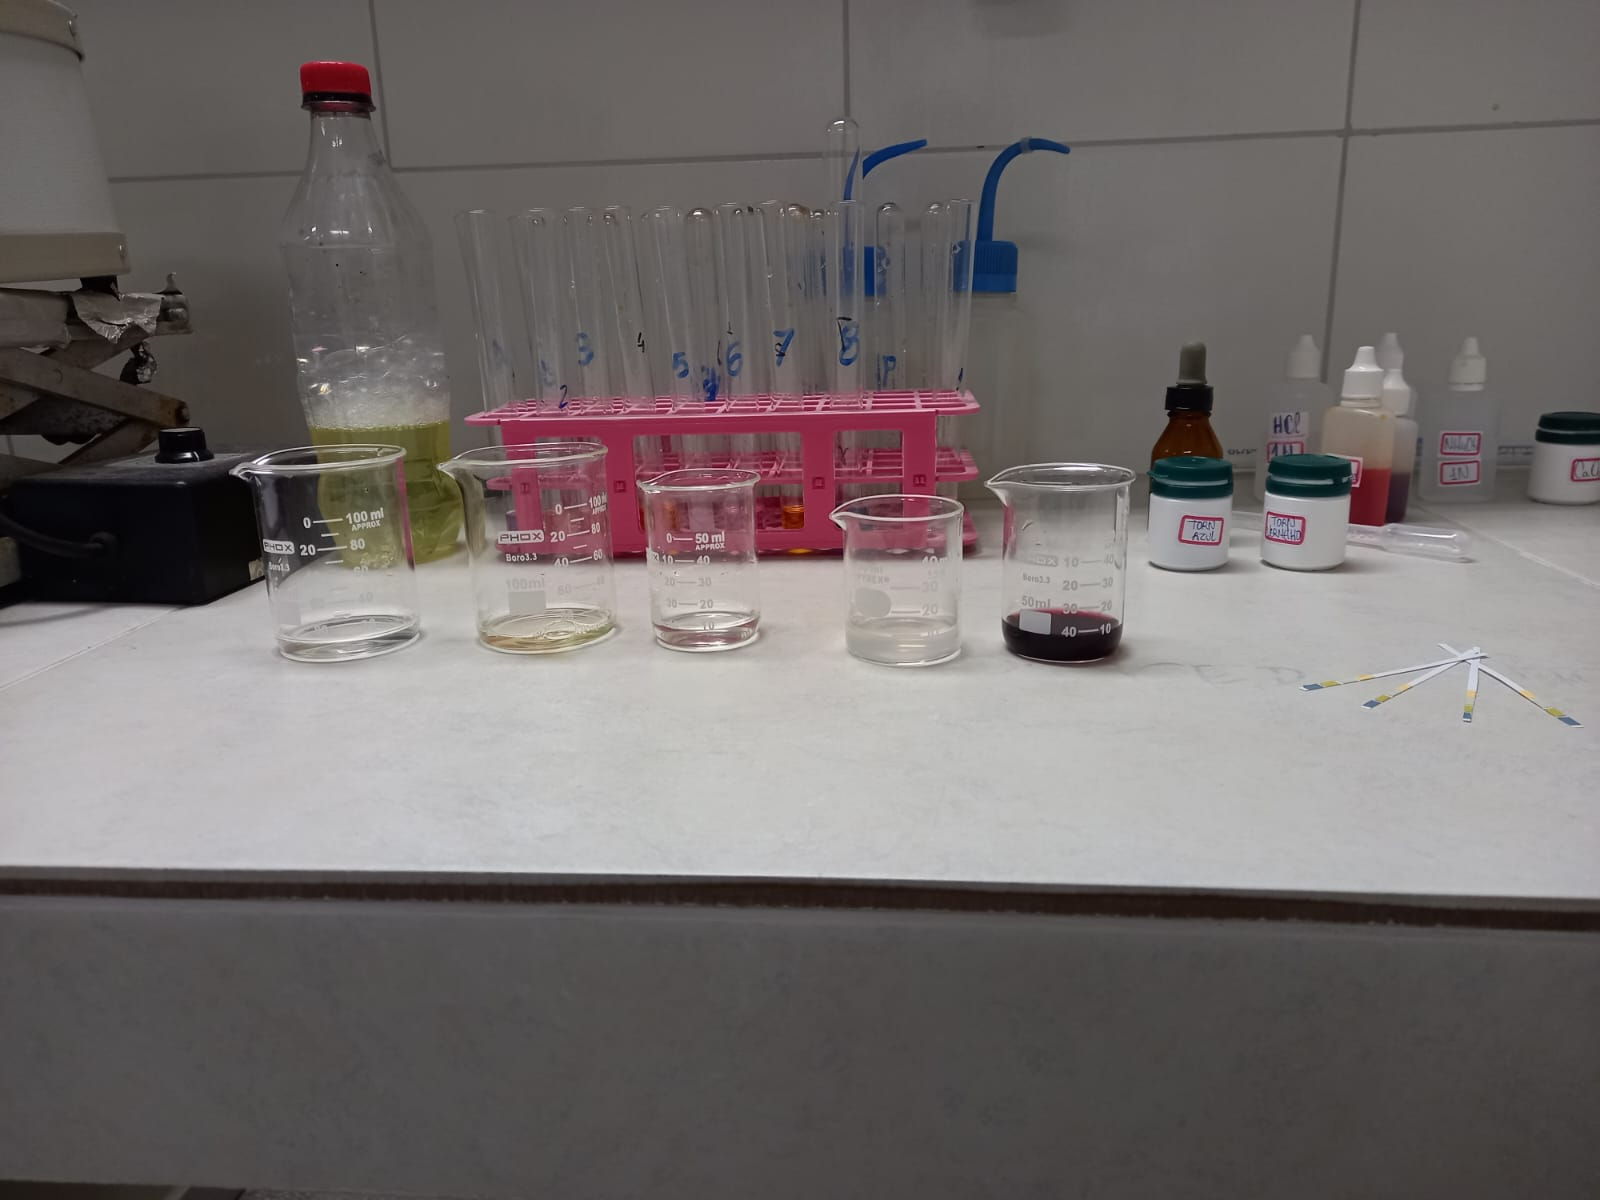
\includegraphics[scale=0.25]{pictures/bancada.jpeg}
        \caption{Bancada de trabalho utilizada para a realização desta prática}\label{fig:figure1}
    \end{figure}\\

    \indent E os materiais de bancada de trabalho utilizadps para a realização desta prática foi composta por:
    \begin{enumerate}
        \item \textbf{8 Tubos de Ensaio} - Utilizados para o preparo das soluções e testes dos indicadores.
        \item \textbf{1 Espátula} - Utilizada para a retirada de amostras das soluções.
        \item \textbf{1 pipeta de 25 mL} - Utilizada para a retirada de amostras das soluções.
        \item \textbf{2 Beckers de 100 mL} - Utilizados para o preparo das soluções.
        \item \textbf{2 Becker de 50 mL} - Utilizado para o preparo das soluções.
        \item \textbf{Estante para tubos de ensaio} - Utilizada para a organização dos tubos de ensaio.
        \item \textbf{Funil de vidro} - Utilizado para o preparo das soluções.
        \item \textbf{Bureta de vidro} - Utilizada para o preparo das soluções.
    \end{enumerate}

    \subsection{Indicadores}\label{subsubsec:mat_materiais_indicadores}
    \indent Muitas substâncias apresentam cores características em determinadas condições, e este é o caso dos indicadores de pH. A exemplo dos indicadores ácidos, estes liberam íons hidroxila (OH$^-$) em solução aquosa, e, portanto, apresentam cores características em soluções ácidas.
    Os indicadores ácidos mais comuns são a fenolftaleína e o bromotimol.
    A fenolftaleína apresenta uma coloração rosa em soluções ácidas e uma coloração incolor em soluções básicas.
    O bromotimol apresenta uma coloração amarela em soluções ácidas e uma coloração azul em soluções básicas.
    Os indicadores ácidos são muito utilizados em laboratórios de química, pois são baratos e fáceis de se obter.
    Além disso, são muito estáveis e apresentam uma boa faixa de pH de coloração.\\
    Portanto, os indicadores ácidos apresentam cores características em soluções ácidas.
    O mesmo ocorre com indicadores básicos e indicadores universais, pois tais compostos irão apresentar cores diferentes em soluções ácidas e básicas.
    Com tudo a depender das concentrações dos íons de (H$^+$) e de (OH$^-$) na solução.

    \section{Métodos}\label{subsec:mat_metodos}
        \indent A experimentação foi realizada seguindo conforme o especificado a seguir:

    \subsection{Experimento 1: Testes dos Indicadores de pH}\label{subsubsec:mat_metodos_exp1}
        \indent Para a realização do experimento 1, foram preparados os tubos de ensaio, cada tubo foi identificado seguindo a numeração de 1 a 8, preparado com suas respectivas soluções para a realização dos testes.\\

        \begin{figure}[h]
            \centering
            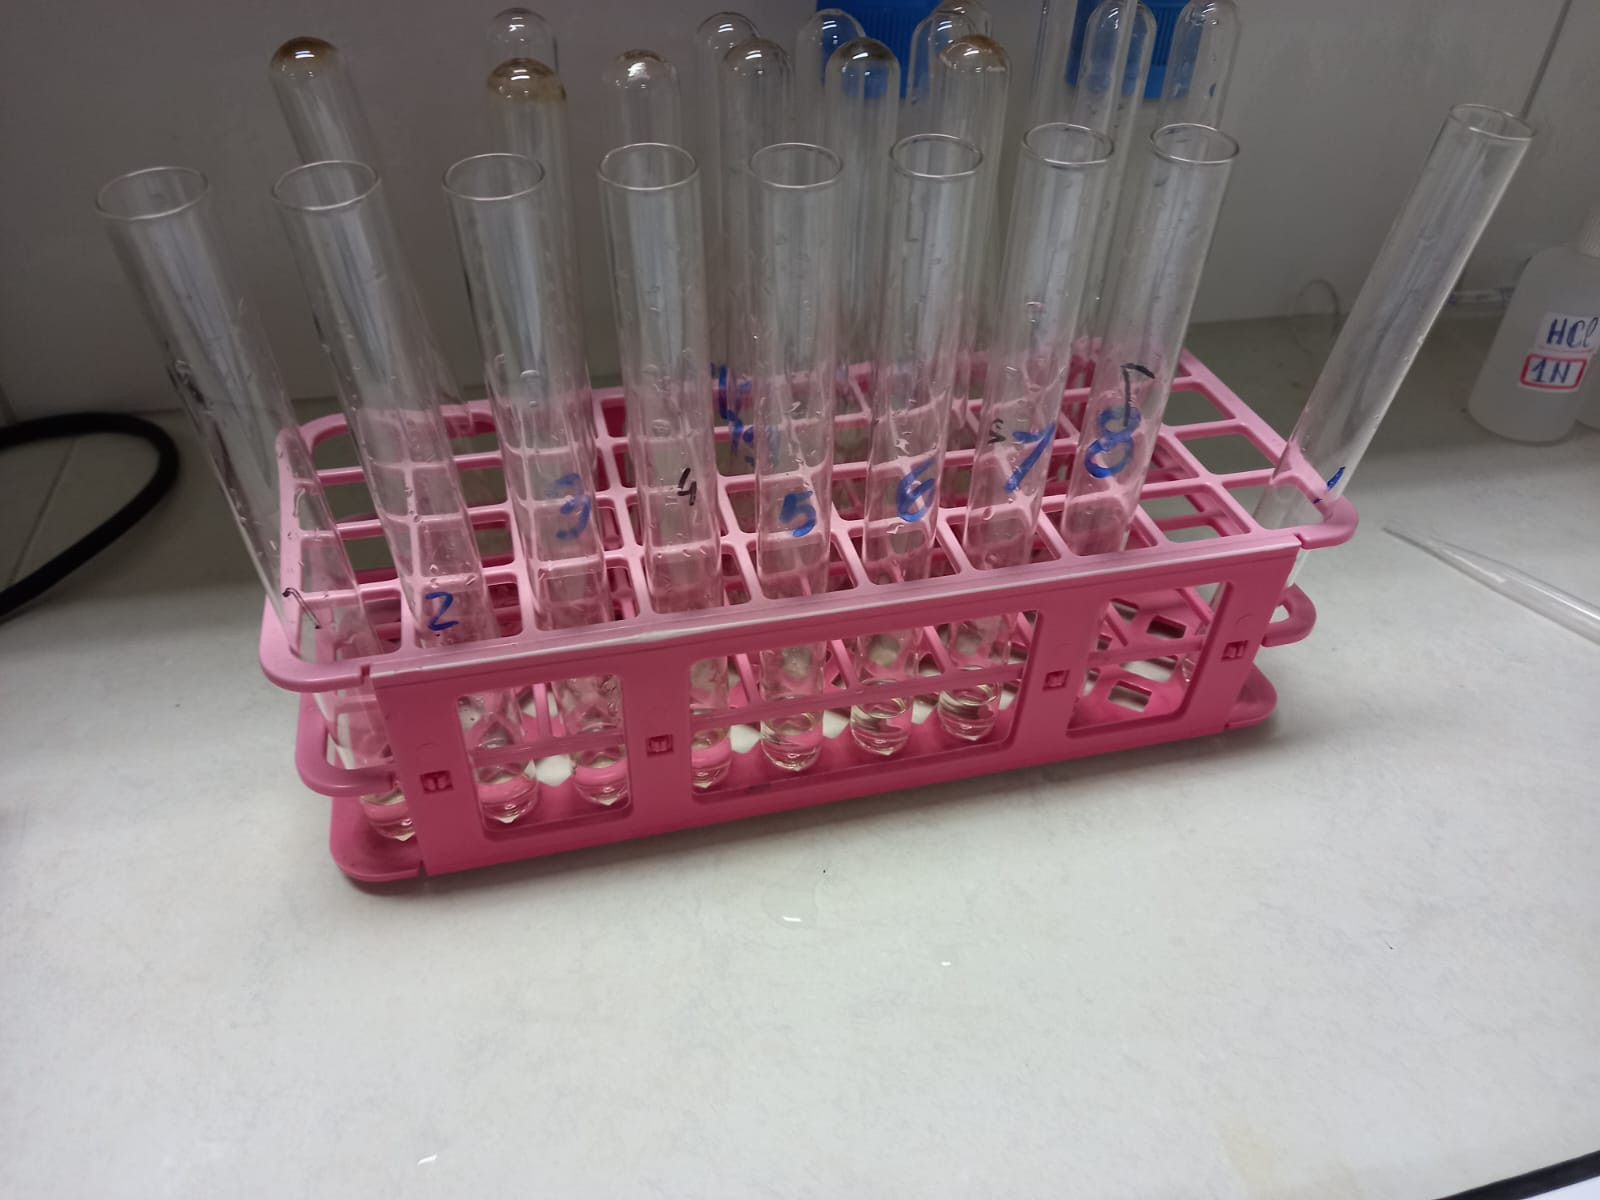
\includegraphics[scale=0.25]{pictures/tubos.jpeg}
            \caption{Tubos de ensaio utilizados para a realização do experimento 1}\label{fig:figure2}
        \end{figure}

        \indent Em suma, os tubos de ensaio foram preparados e testados com os indicadores, seguindo a tabela a seguir, cada experimentação será descrita detalhadamente posteriormente.\\

        \newpage

        \begin{table}[h]\label{tab:tubos}
            \label{tab:experimento1}
            \centering
            \begin{tabular}{|c|c|c|c|c|c|c|c|}
                \hline
                \textbf{Tubo} & \textbf{Solução} & \textbf{Indicador} & \textbf{Cor Apresentada}\\
                \hline
                1 & Solução de NaOH 0,1 mol/L & Papel Tornassol - Azul & Cristalino azulado \\
                \hline
                2 & Solução de HCl 0,1 mol/L & Papel Tornassol - Azul & Cristalino azulado \\
                \hline
                3 & Solução de CH$_3$COOH 0,1 mol/L & Alaranjado de Metila & Alaranjado\\
                \hline
                4 & Solução de NH$_4$OH 0,1 mol/L & Alaranjado de Metila & Amarelo \\
                \hline
                5 & Solução de HCl 0,1 mol/L & Fenolftaleína & Branco \\
                \hline
                6 & Solução de NaOH 0,1 mol/L & Fenolftaleína & Rosa / Magenta \\
                \hline
                7 & Solução de CH$_4$COOH 0,1 mol/L & Azul de Bromotimol & Amarelo \\
                \hline
                8 & Solução de NH$_4$OH 0,1 mol/L & Azul de Bromotimol & Azul \\
                \hline
            \end{tabular}
            \caption{Tabela de experimento 1}
        \end{table}
		
	\subsubsection{Tubo de Ensaio 1}
        \indent O primeiro tubo foi preparado com a solução de NaOH 0,1 mol/L, e foi testado com o indicador de pH, o papel de tornassol azul, o qual apresentou uma cor cristalina azulada.\\
        
	\subsubsection{Tubo de Ensaio 2}
        \indent O segundo tubo foi preparado com a solução de HCl 0,1 mol/L, e foi testado com o indicador de pH, o papel de tornassol vermelho, o qual apresentou uma cor cristalina azulada, os comportamentos dos tubos 1 e 2 podem ser visualizados conforme a figura a seguir:\\

        \begin{figure}[h]
            \centering
            \subfloat[\centering Teste do indicador de pH com as soluções de NaOH e HCl de 0,1 mol/L\label{fig:figure3}]{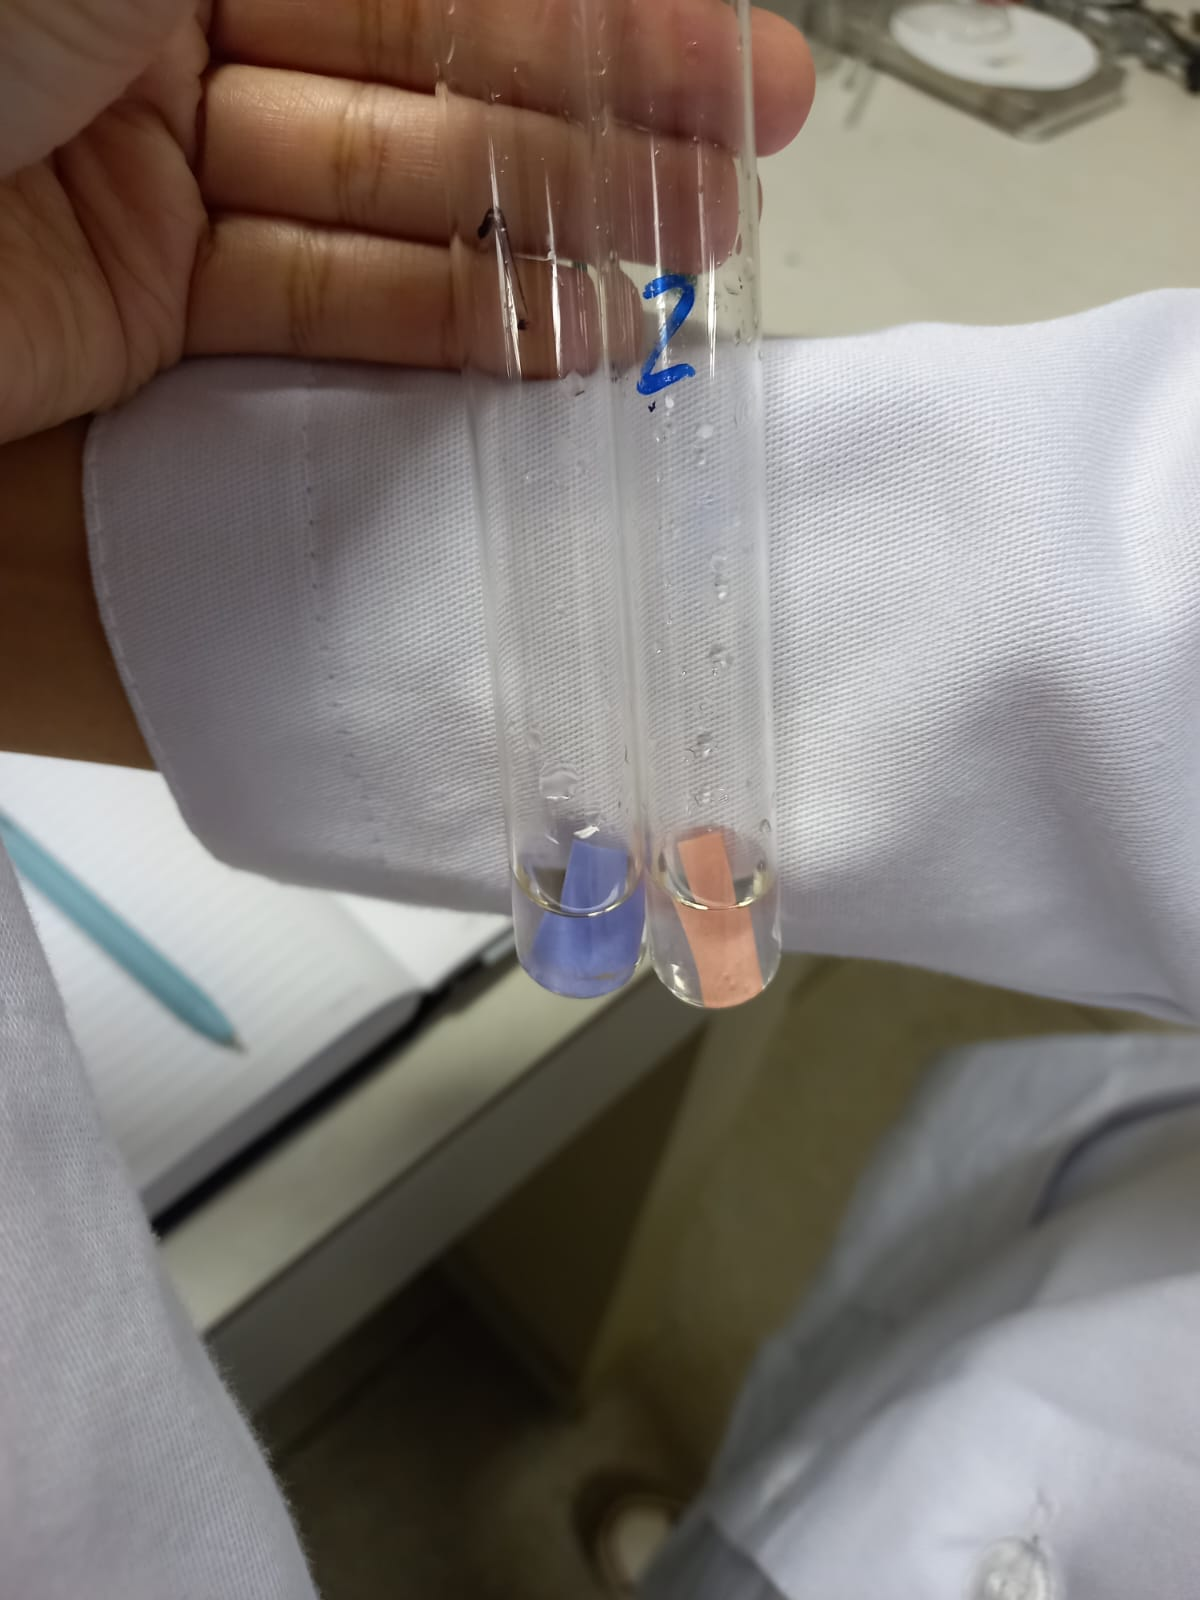
\includegraphics[scale=0.16]{pictures/tubo1e2pre.jpeg}}
            \qquad
            \subfloat[\centering Teste com as soluções com a adição dos papéis azul e vermelho em ambos os tubos. \label{fig:figure4}]{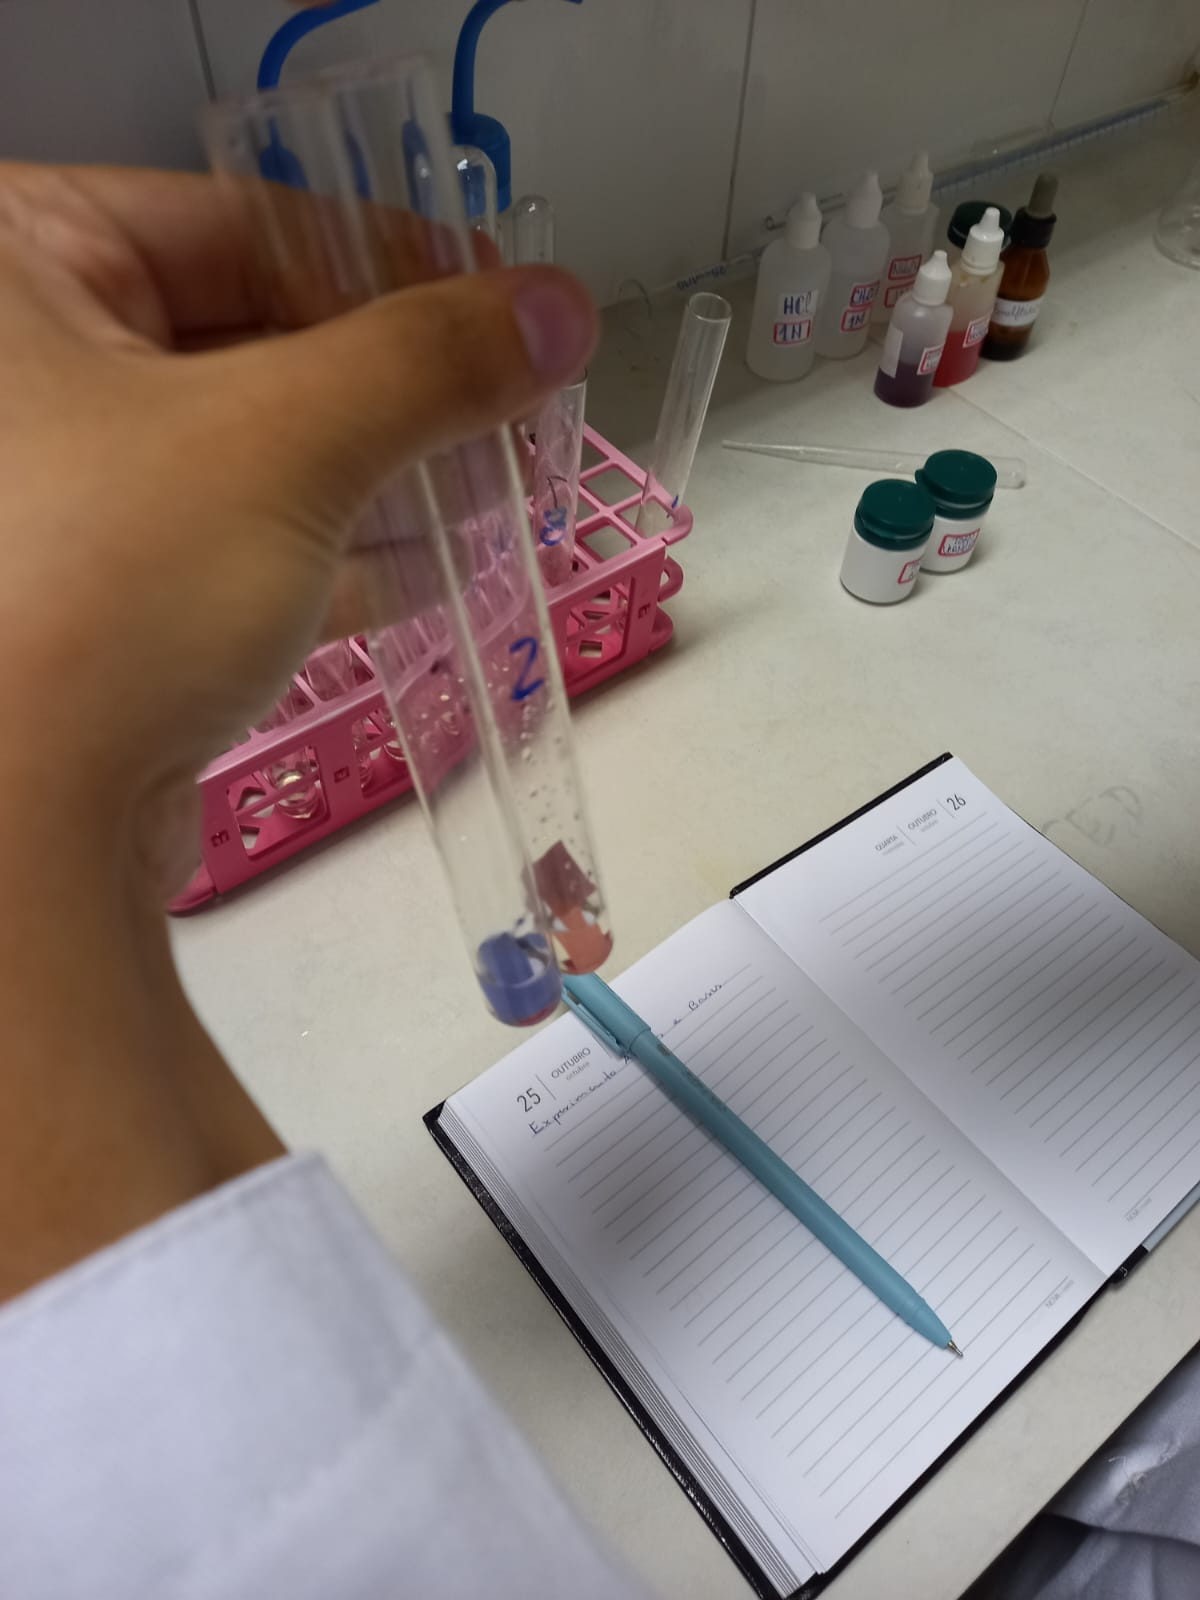
\includegraphics[scale=0.16]{pictures/tubo1e2pos.jpeg}}
            \caption{Teste do indicador de pH, o papel de tornassol azul e vermelho, nos tubos 1 e 2}\label{fig:experimento11}
        \end{figure}

        \indent O papel tornassol é muito utilizado em avaliações qualitativas de pH, é conhecido que seu comportamento é de tornar-se vermelho em soluções com pH abaixo de 4,7 e azul em soluções com pH acima de 8,3. Foi observado que, quando um papel azul é exposto à uma solução ácida, este se torna vermelho, e quando exposto à uma solução básica, nada acontece, e quando um papel vermelho é exposto em uma solução básica, este torna-se azul, mas quando exposto à solução ácida, nada acontece.\\
        
	\subsubsection{Tubo de Ensaio 3}
        \indent O terceiro tubo foi preparado com a solução de CH$_3$COOH 0,1 mol/L, e foi testado com o indicador de pH, o alaranjado de metila, o qual apresentou uma cor alaranjada.

        \begin{figure}[h]
            \centering
            \subfloat[\centering Teste do indicador de pH com a solução de CH$_3$COOH de 0,1 mol/L\label{fig:figure5}]{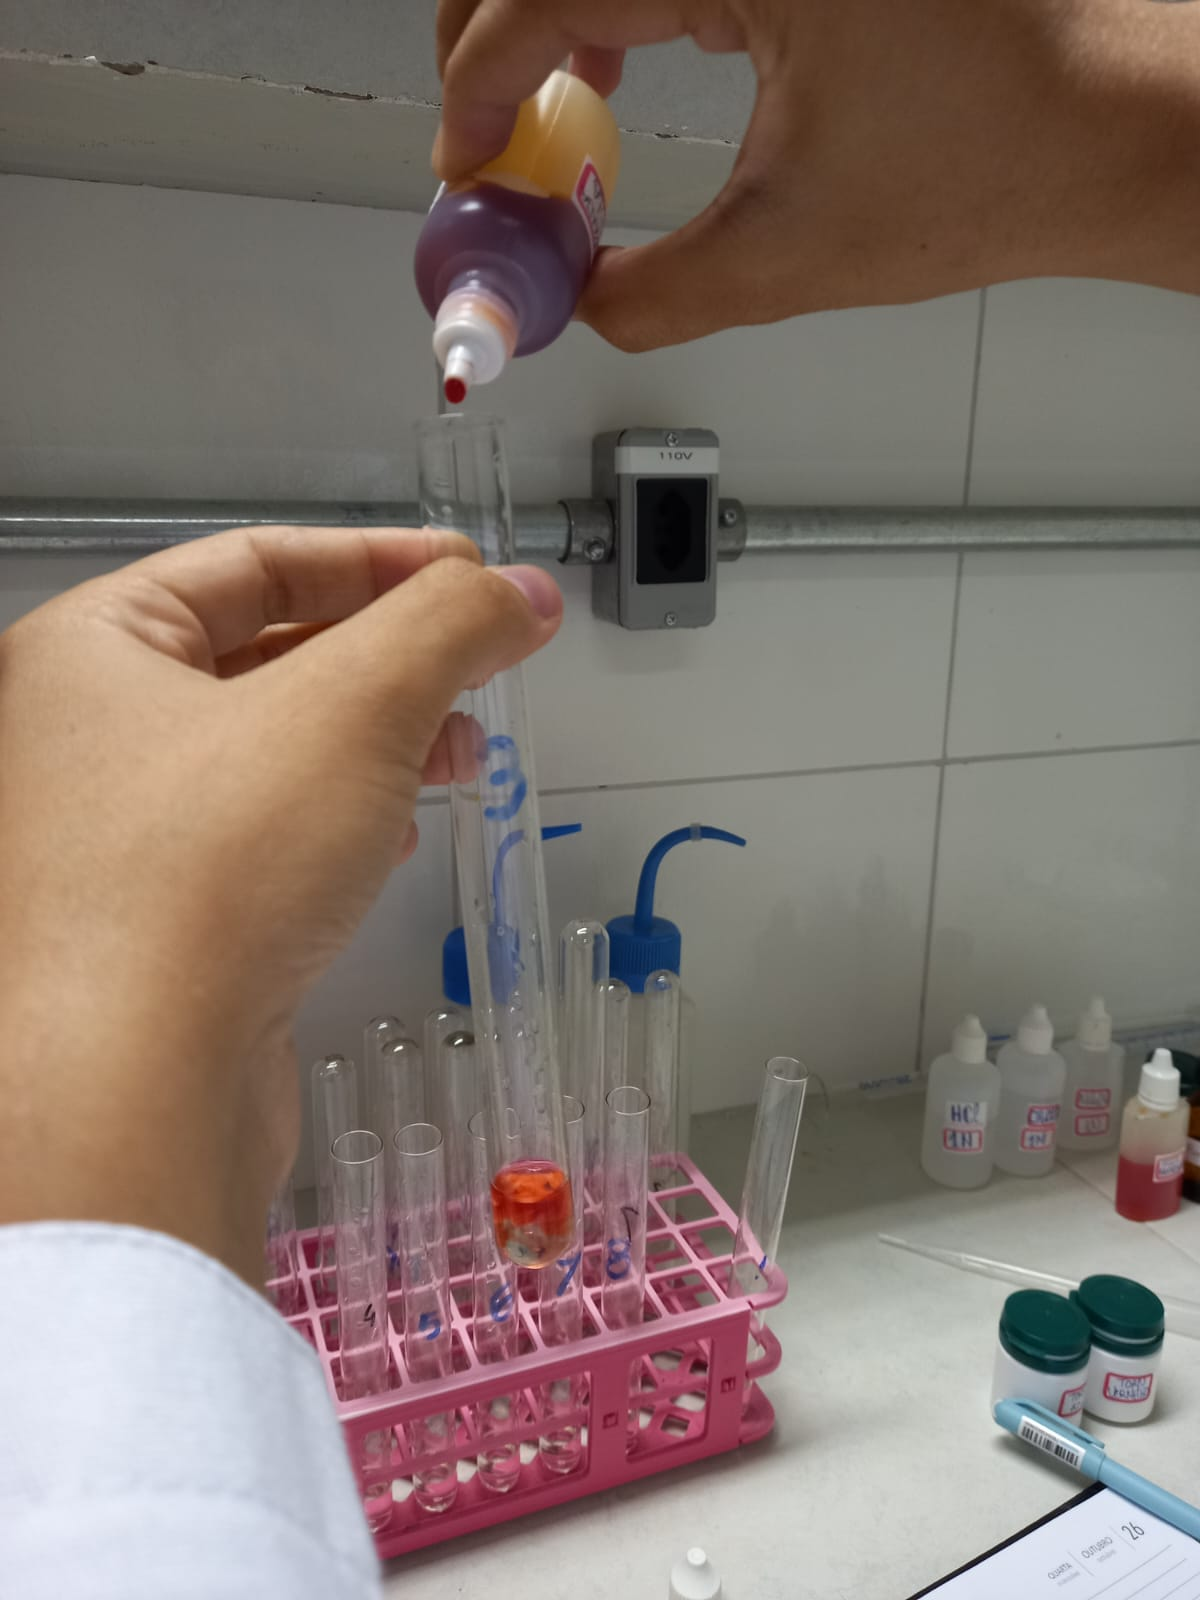
\includegraphics[scale=0.16]{pictures/tubo3pre.jpeg}}
            \qquad
            \subfloat[\centering A coloração apresentadapelo indicador foi alaranjada.\label{fig:figure6}]{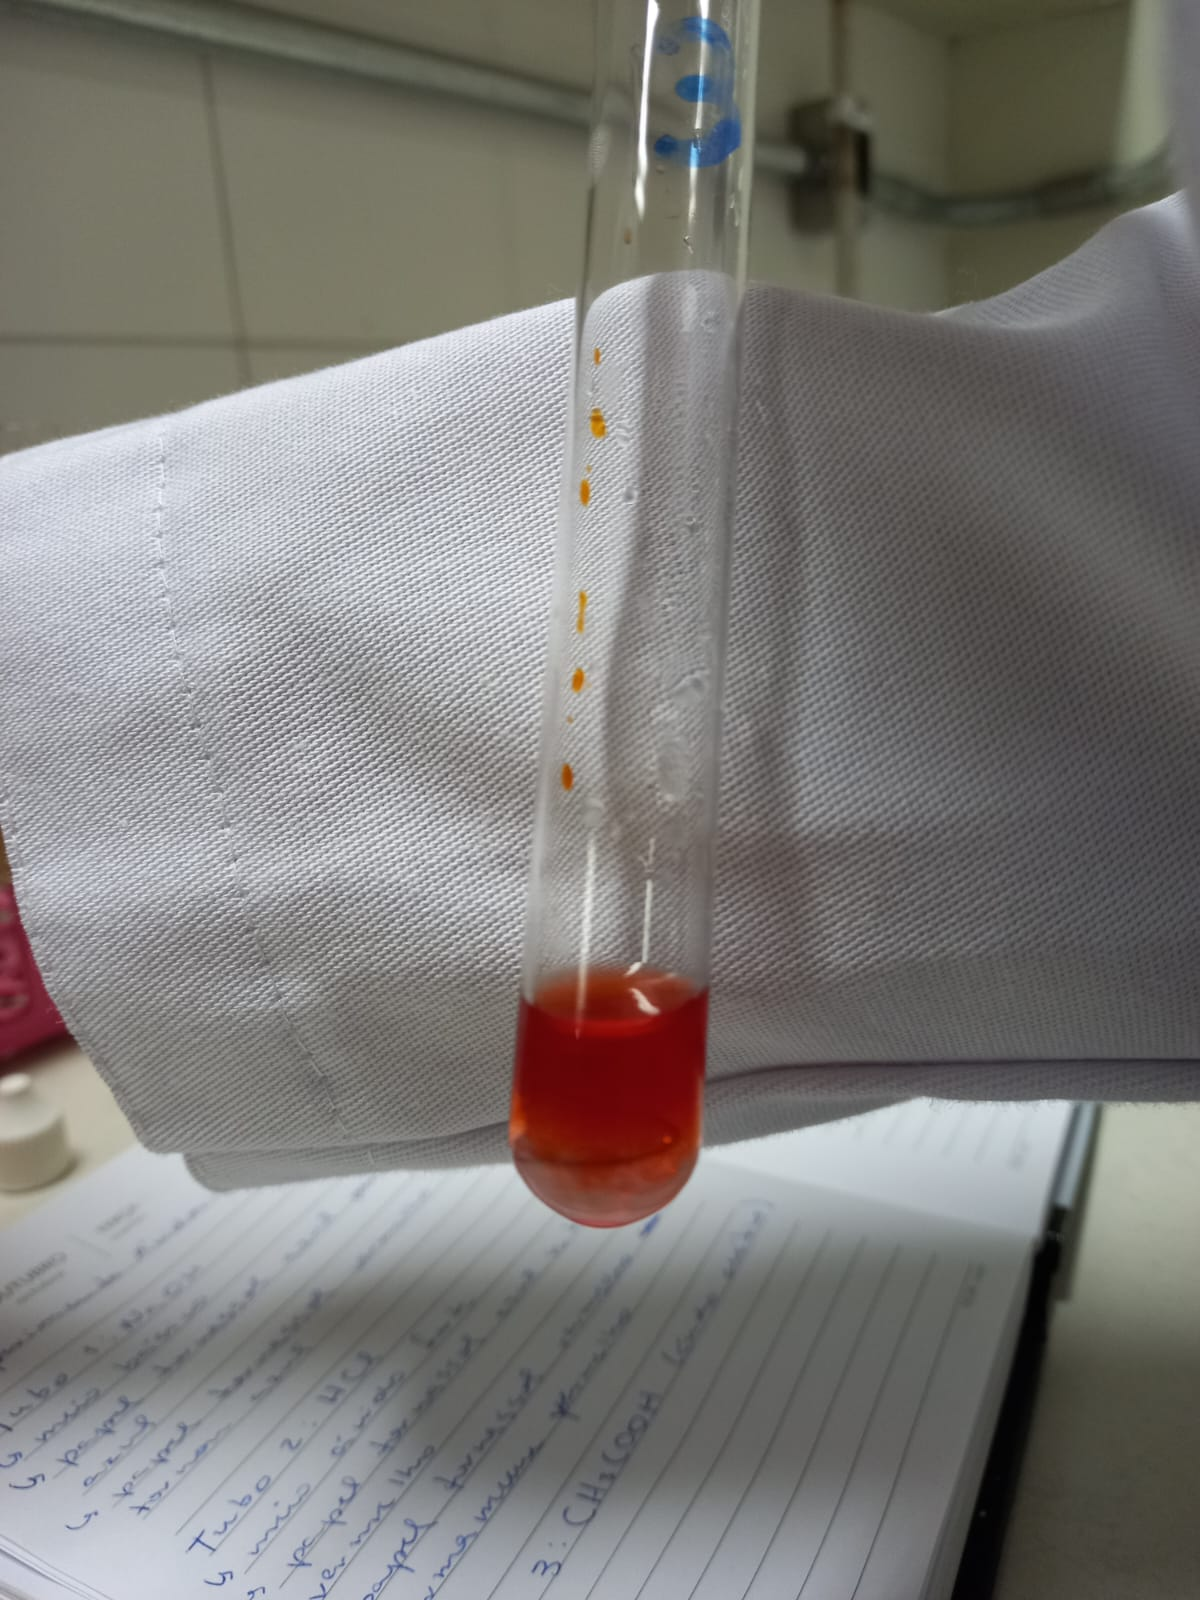
\includegraphics[scale=0.16]{pictures/tubo3pos.jpeg}}\label{fig:experimento12}
        \end{figure}
    	
    	\indent O alaranjado de metila é um indicador para ácidos, em que sua coloração varia desde um vermelho intenso para pHs abaixo de 3,1 e amarelo para pHs superiores a 4,4. Logo, ao comparar sua tabela de cores com a coloração obtida no experimento realizado com o ácido acético, podemos observar que o pH apresentado pela solução está abaixo de 4,4, mas mais próximo do limite superior (4,4), do que do limite inferior (3,1) de coloração da solução pelo indicador.\\

	\newpage
	\subsubsection{Tubo de Ensaio 4}

        \indent O quarto tubo foi preparado com a solução de NH$_4$OH 0,1 mol/L, e foi testado com o indicador de pH, o alaranjado de metila, o qual apresentou uma cor branca.

        \begin{figure}[h]
            \centering
            \subfloat[\centering Teste do indicador de pH com a solução de NH$_4$OH de 0,1 mol/L\label{fig:figure7}]{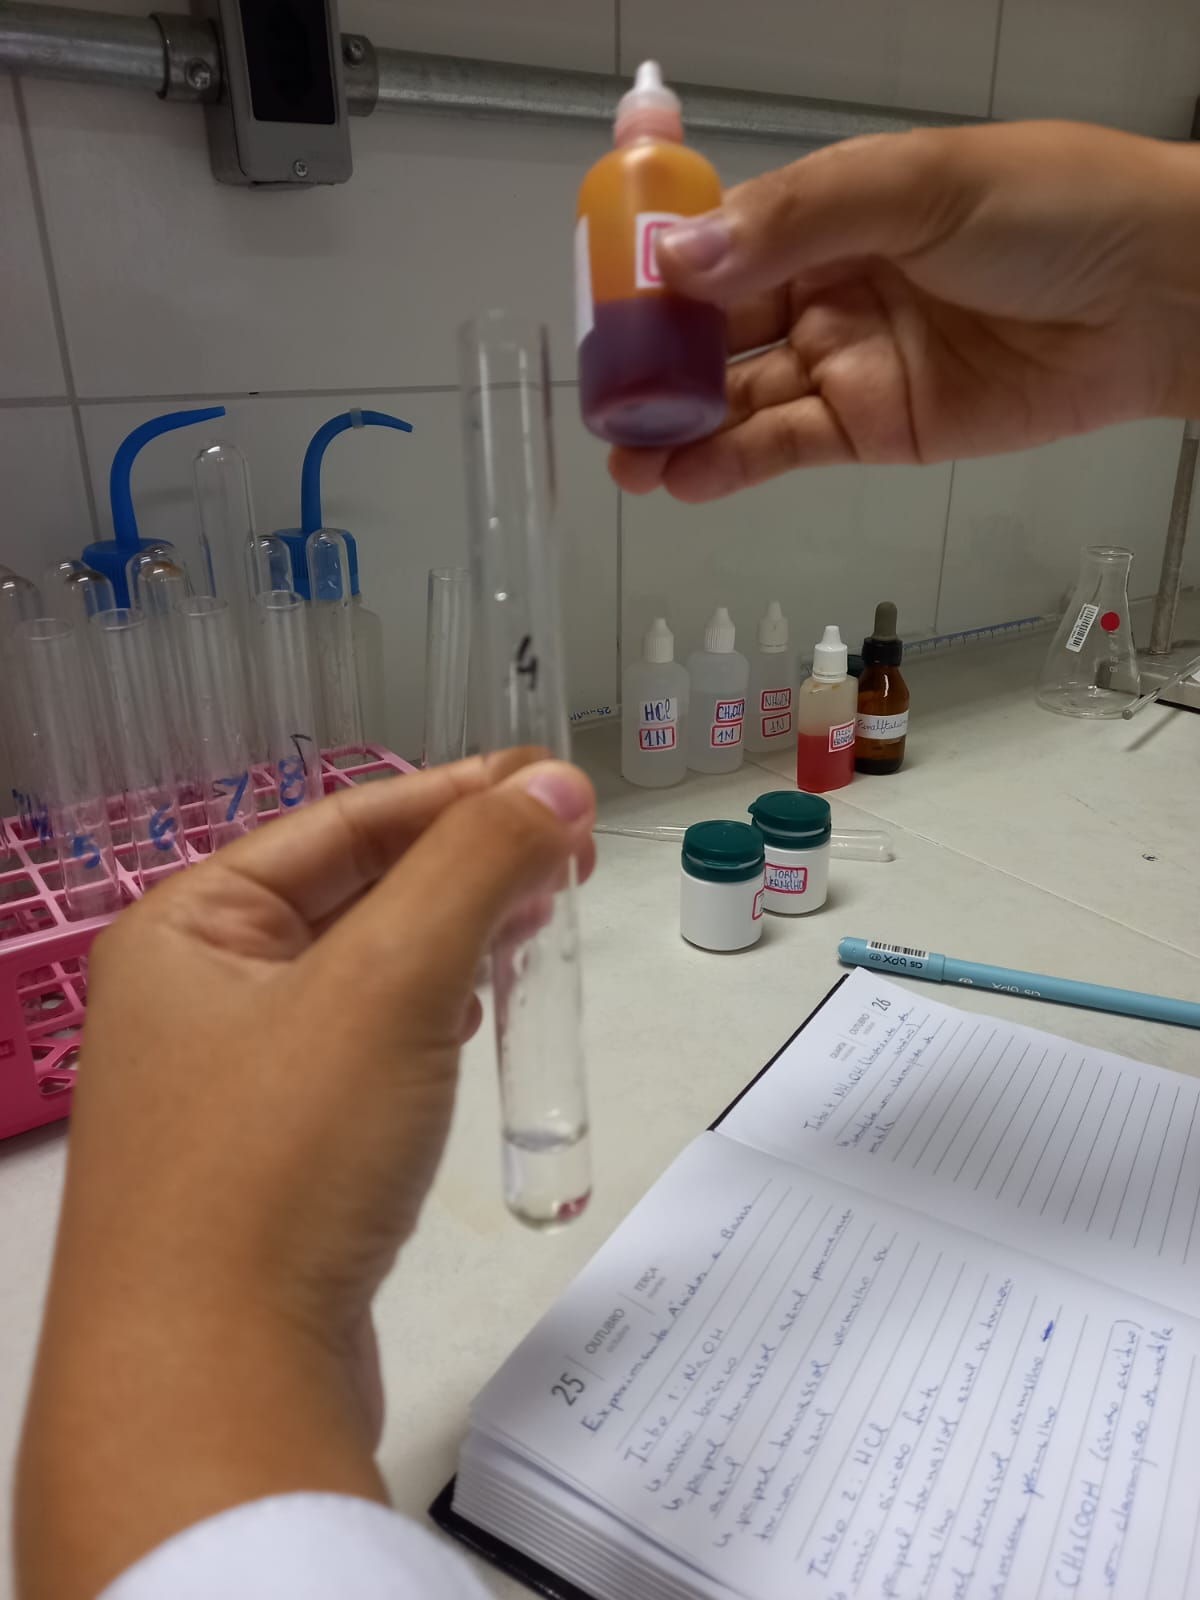
\includegraphics[scale=0.16]{pictures/tubo4pre.jpeg}}
            \qquad
            \subfloat[\centering A coloração apresentada pelo indicador foi uma tonalidade amarela. \label{fig:figure8}]{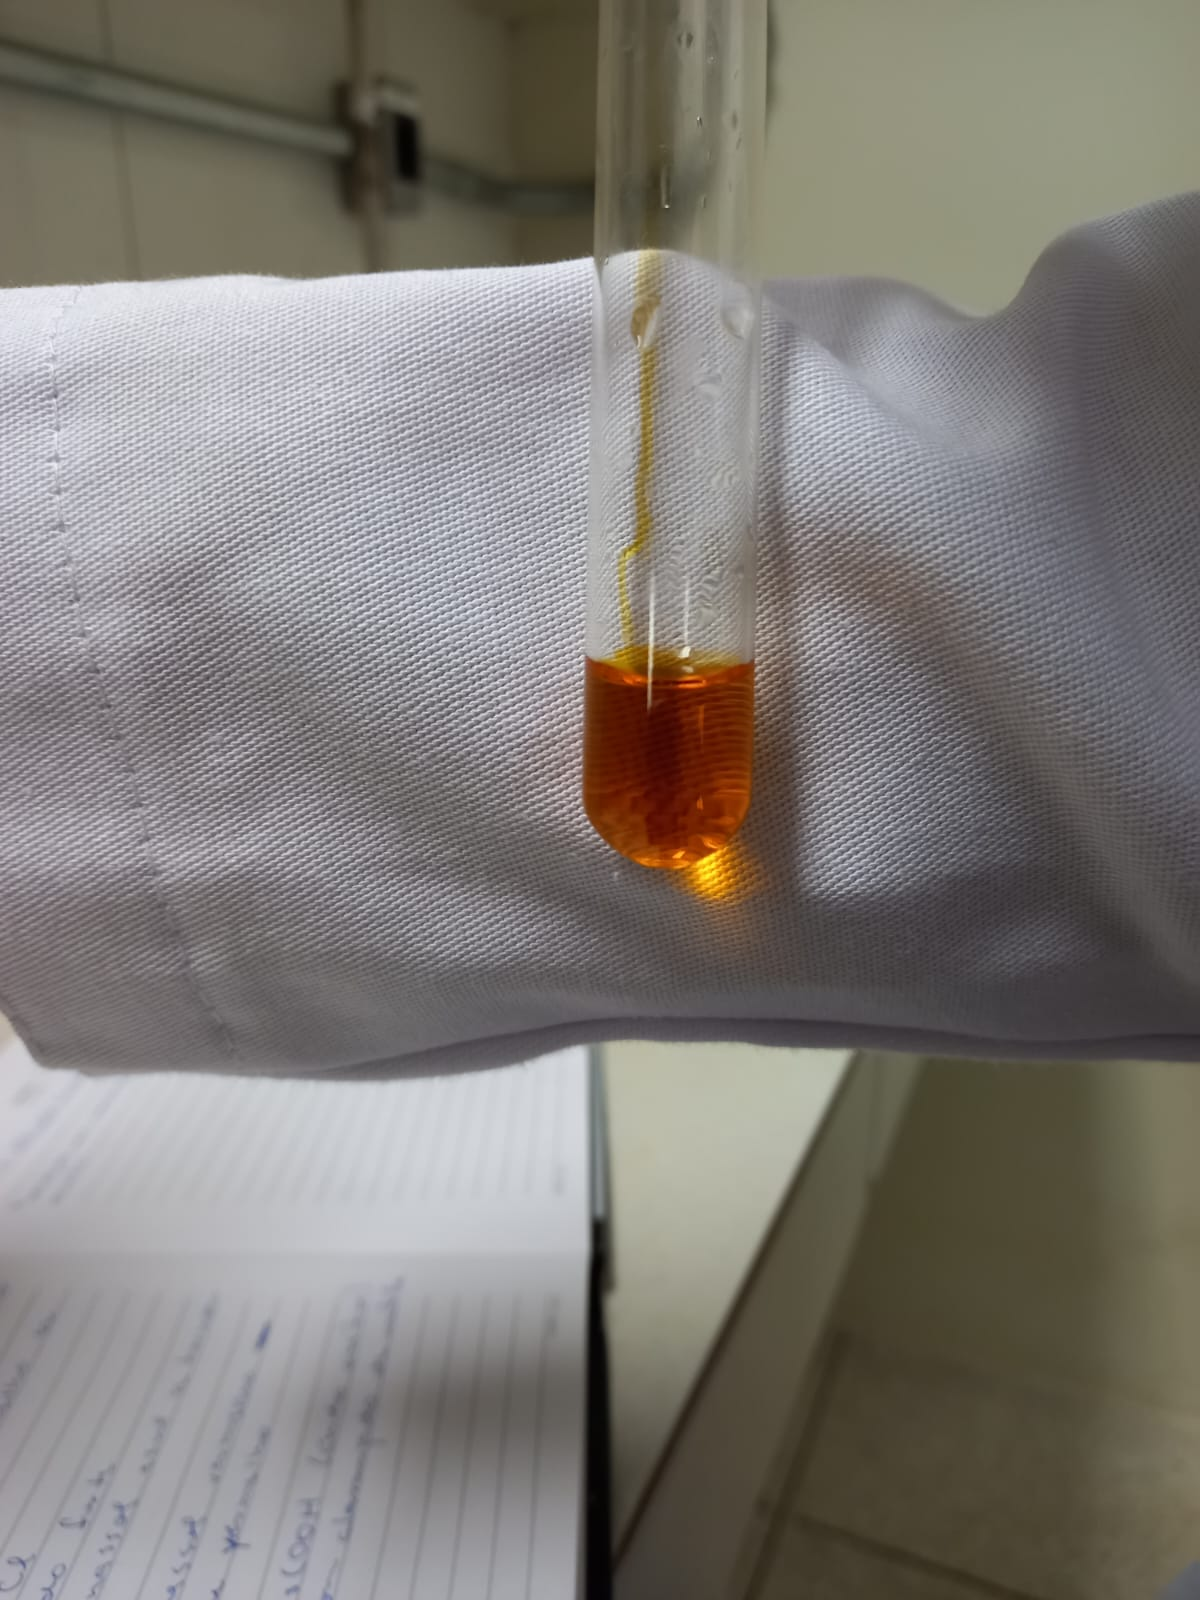
\includegraphics[scale=0.16]{pictures/tubo4pos.jpeg}}\label{fig:experimento13}
        \end{figure}
    	
    	\indent Neste experimento, foi realizado o teste do hidróxido de amônio. Como exemplificado no ensaio do tubo 3, o alaranjado de metila apresenta variação de cores até pH 4,4, após este limite, o mesmo apresenta uma coloração amarelada por padrão. Tal comportamento foi observado neste experimento, sendo apenas possível determinar que o pH desta solução é superior a 4,4. \\
    	
    	\indent Neste caso em específico, é fato conhecido que o hidróxido de amônio é um composto químico com forte caráter básico, e portanto, o indicador alaranjado de metila não é um bom indicador para o estudo de pH da solução em questão.\\
    	
    \newpage

    \subsubsection{Tubo de Ensaio 5}

        \indent O quinto tubo foi preparado com a solução de HCl 0,1 mol/L, e foi testado com o indicador de pH, a fenolftaleína, o qual apresentou uma cor rosa.\\

        \begin{figure}[ht]
            \centering
                \subfloat[\centering Teste do indicador de pH com a solução de HCl de 0,1 mol/L\label{fig:figure9}]{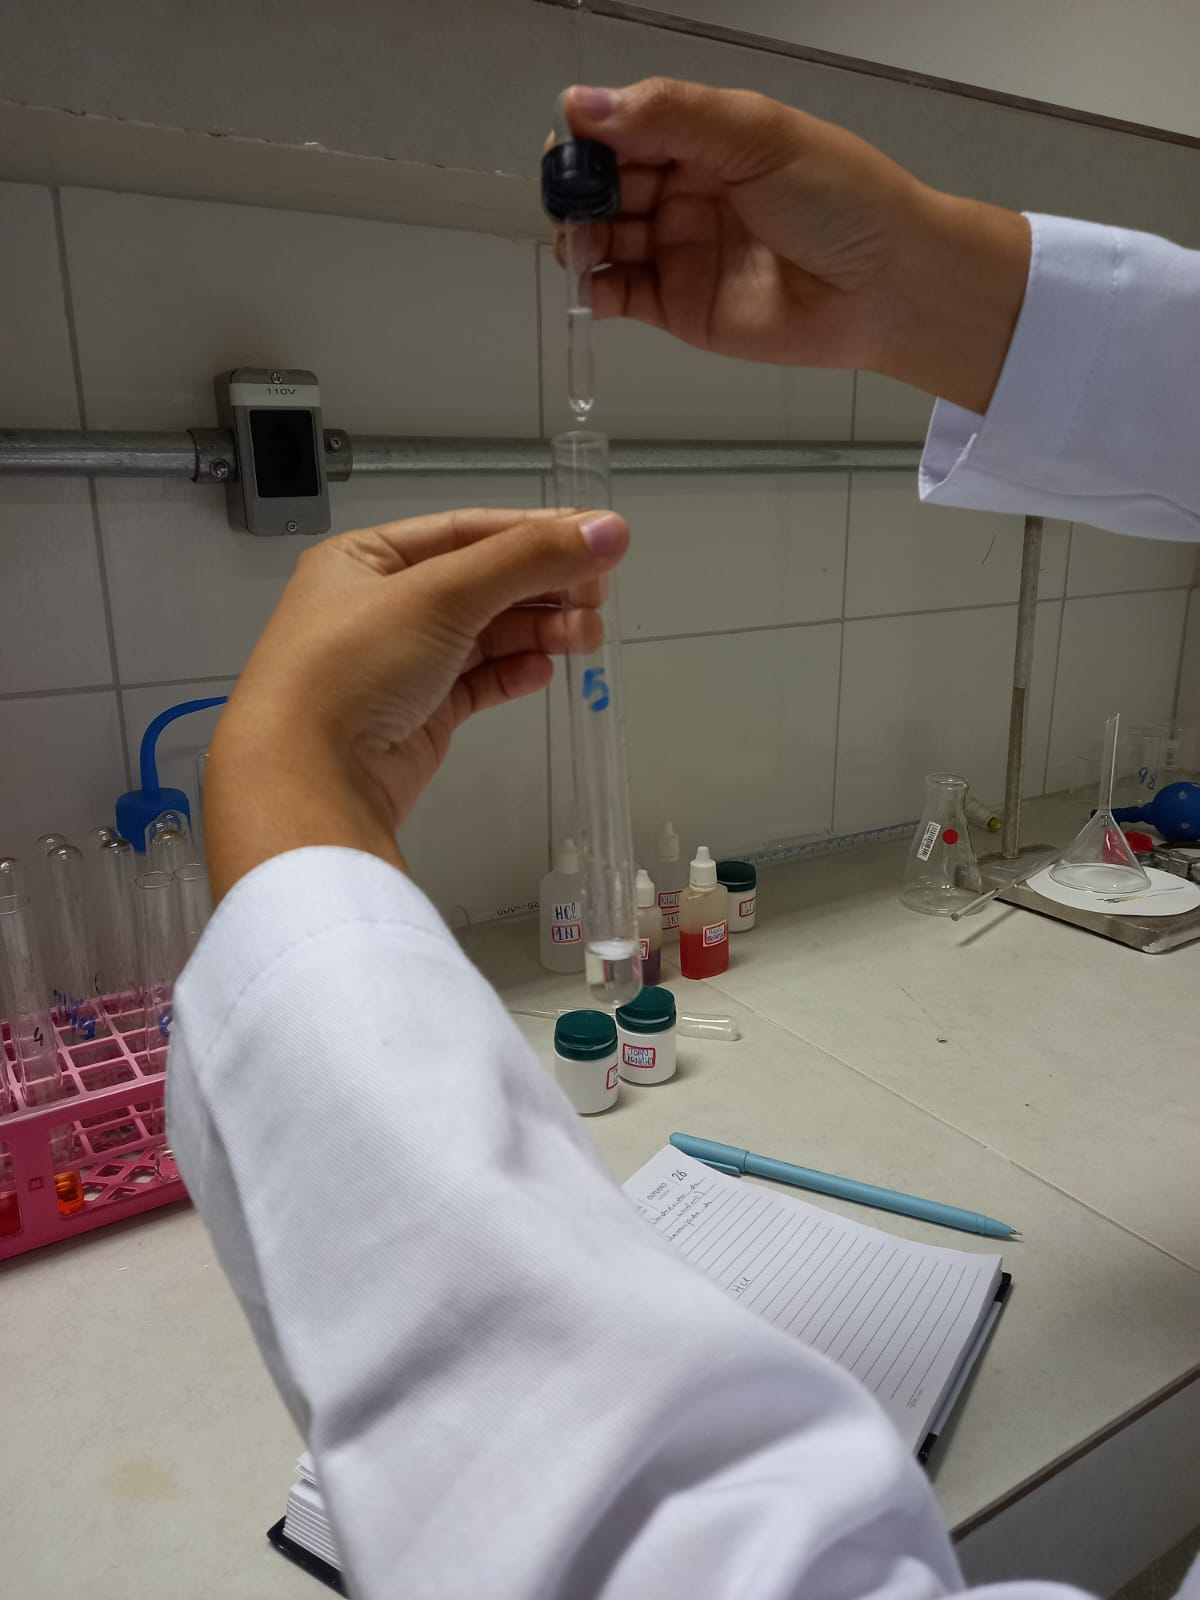
\includegraphics[scale=0.16]{pictures/tubo5pre.jpeg}}
                \qquad
                \subfloat[\centering A coloração apresentada pelo indicador foi branca.\label{fig:figure10}]{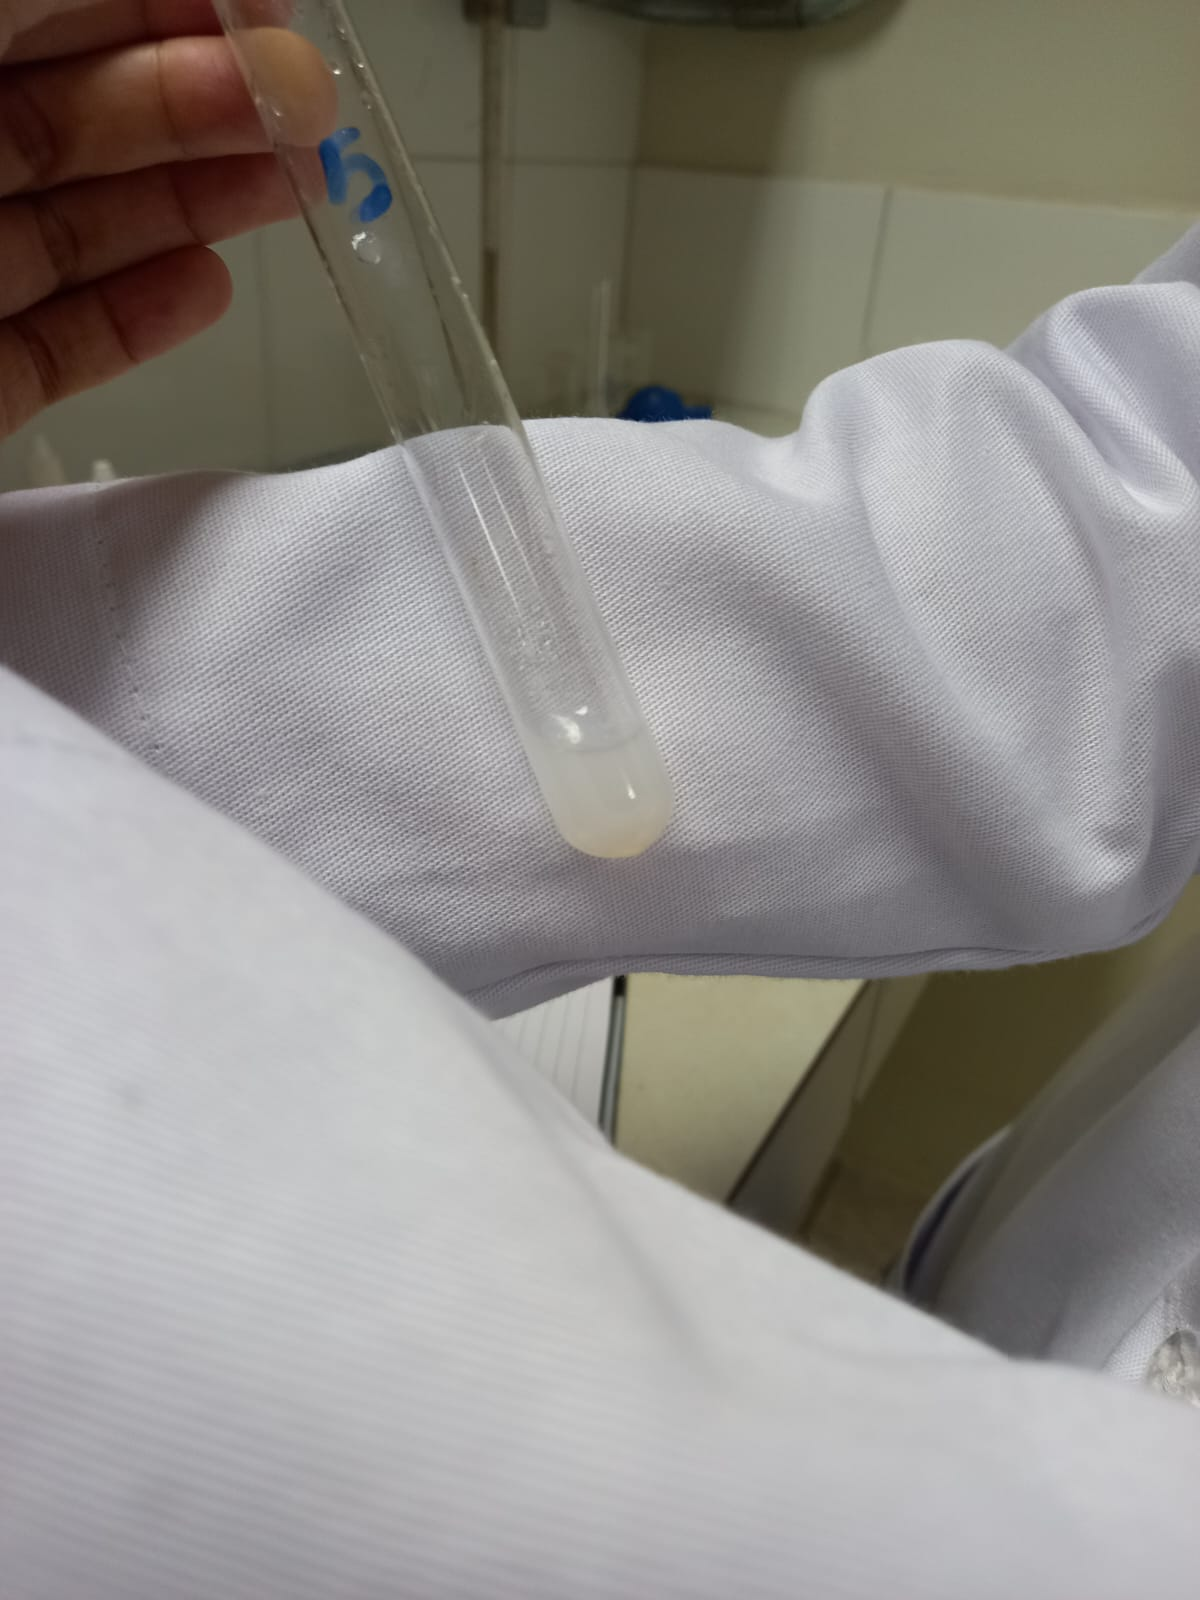
\includegraphics[scale=0.16]{pictures/tubo5pos.jpeg}}\label{fig:experimento14}
        \end{figure}
		
		\indent Neste ensaio, os testes foram realizados com o indicador fenolftaleína, este indicador é utilizado para a detecção de bases, apresentando tonalidade roxa / magenta para pHs a cima de 10, tonalidade rosa para pHs entre 8 e 10, e branco / incolor para pHs abaixo de 8.\\
		
		\indent Neste experimento, foi utilizado o ácido clorídrico, e no teste, a tonalidade apresentada foi um turvo esbranquiçado. Esperava-se que a solução demonstrasse um aspécto incolor, porém, os motivos desta ter adquirido a tonalidade branca ao invés de ser incolor não foram bem compreendidos.\\
			
		\indent A fenolftaleína é um indicador para bases, uma vez que sua sensibilidade ao pH da solução é relativa a valores superiores a 8, portanto, este indicador não é o mais adequado para testes com soluções de caráter ácido.
		
	\newpage
	\subsubsection{Tubo de Ensaio 6}

        \indent O sexto tubo foi preparado com a solução de NaOH 0,1 mol/L, e foi testado com o indicador de pH, a fenolftaleína, o qual apresentou uma solução incolor.
        \begin{figure}[h]
            \centering
            \subfloat[\centering Teste do indicador de pH com a solução de NaOH de 0,1 mol/L\label{fig:figure11}]{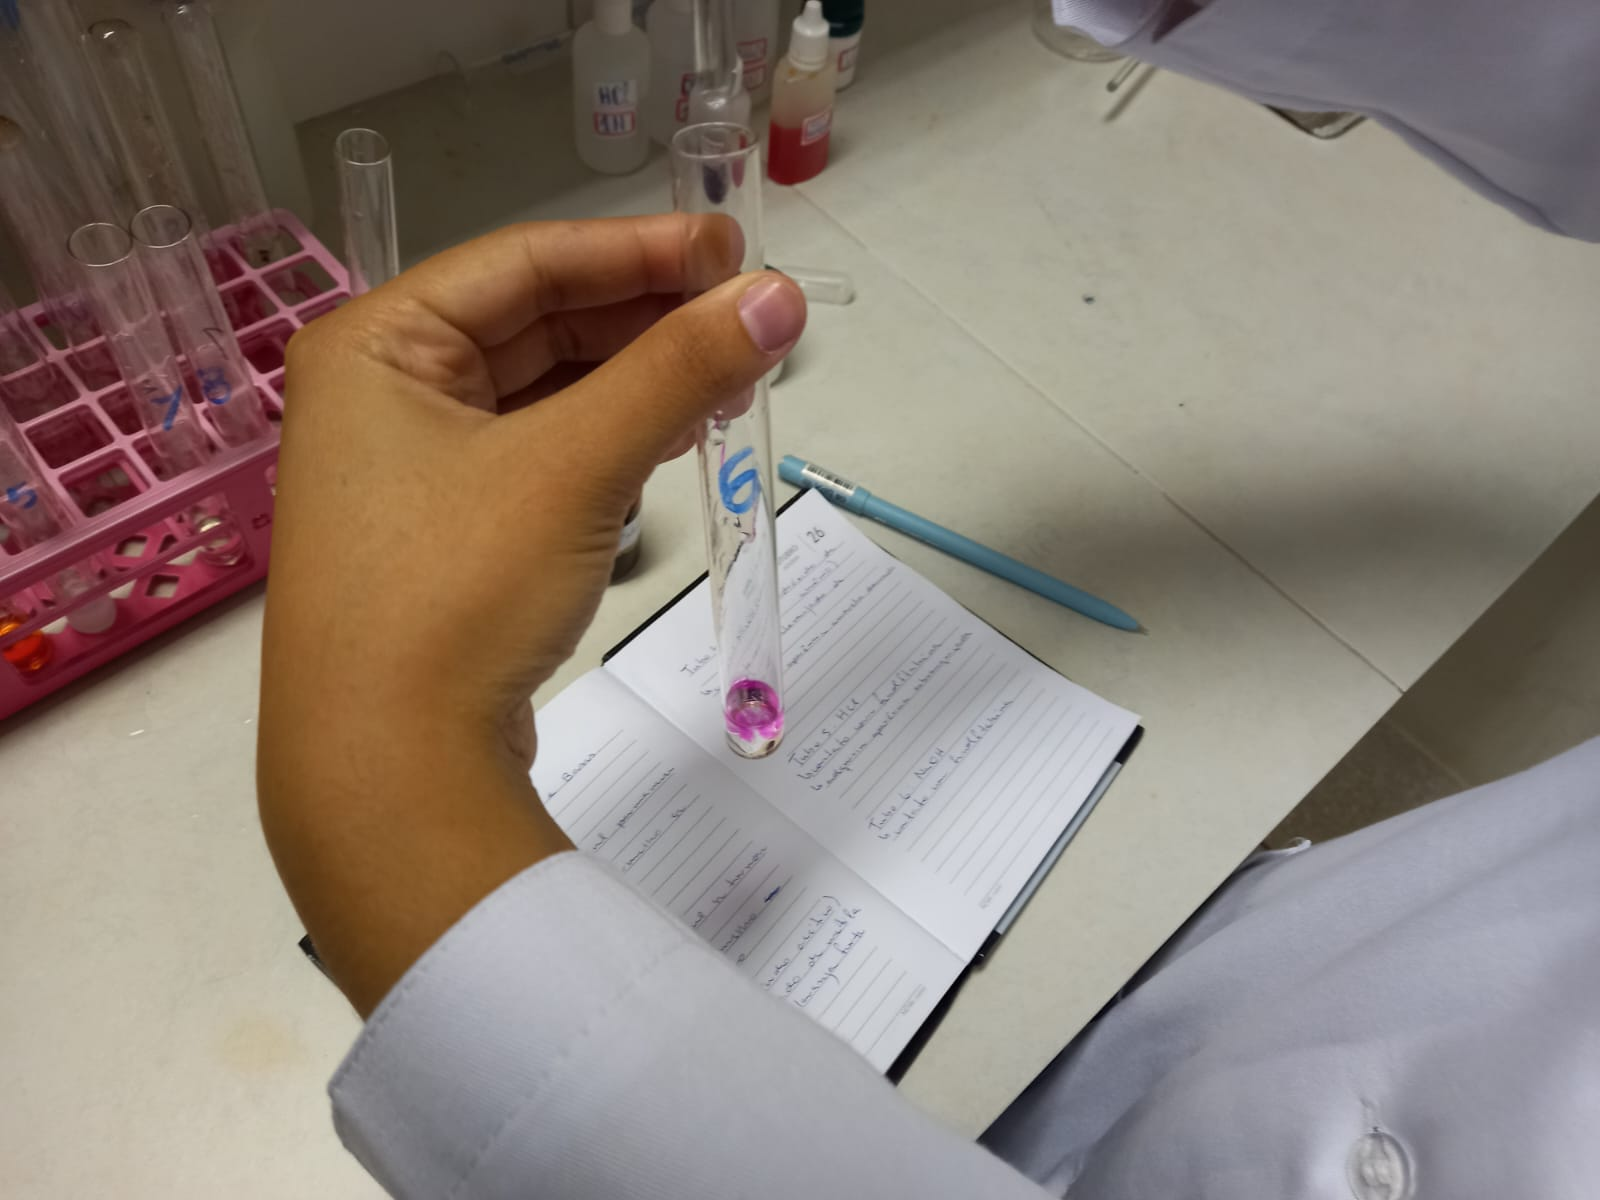
\includegraphics[scale=0.20]{pictures/tubo6pre.jpeg}}
            \qquad
            \subfloat[\centering A coloração apresentada pelo indicador foi rosa magenta.\label{fig:figure12}]{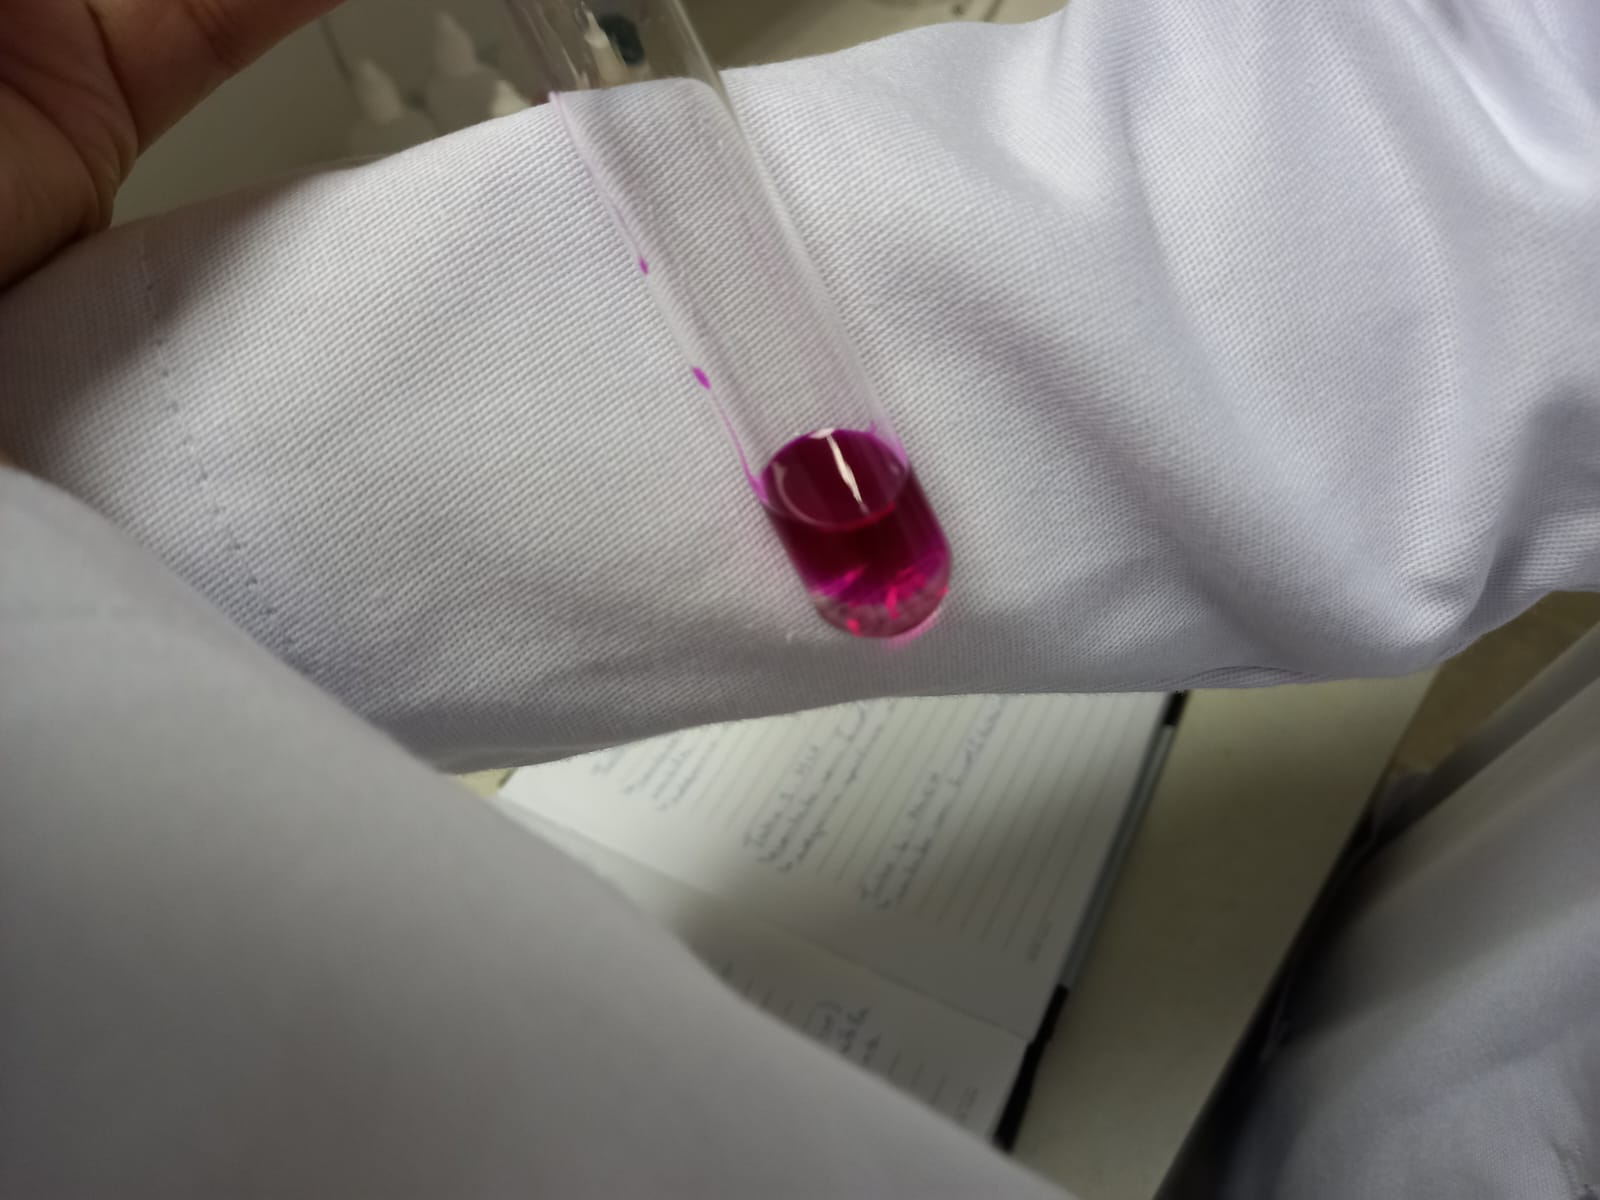
\includegraphics[scale=0.20]{pictures/tubo6pos.jpeg}}\label{fig:experimento15}
        \end{figure}
    
    	\indent Este ensaio foi preparado com uma solução de hidróxido de sódio e testado com fenolftaleína, portanto, ao entrar em contato com uma base forte, o indicador mudou a sua coloração para uma tonalidade magenta.\\
    	
    	\indent Com a visualização da cor, foi possível determinar que o pH apresentado por esta solução é superior a 10.

	\newpage
	\subsubsection{Tubo de Ensaio 7}

        \indent O sétimo tubo foi preparado com a solução de CH$_3$COOH 0,1 mol/L, e foi testado com o indicador de pH, o azul de bromotimol, o qual apresentou uma cor amarelada.

        \begin{figure}[h]
            \centering
            \subfloat[\centering Teste do indicador de pH com a solução de CH$_3$COOH de 0,1 mol/L\label{fig:figure13}]{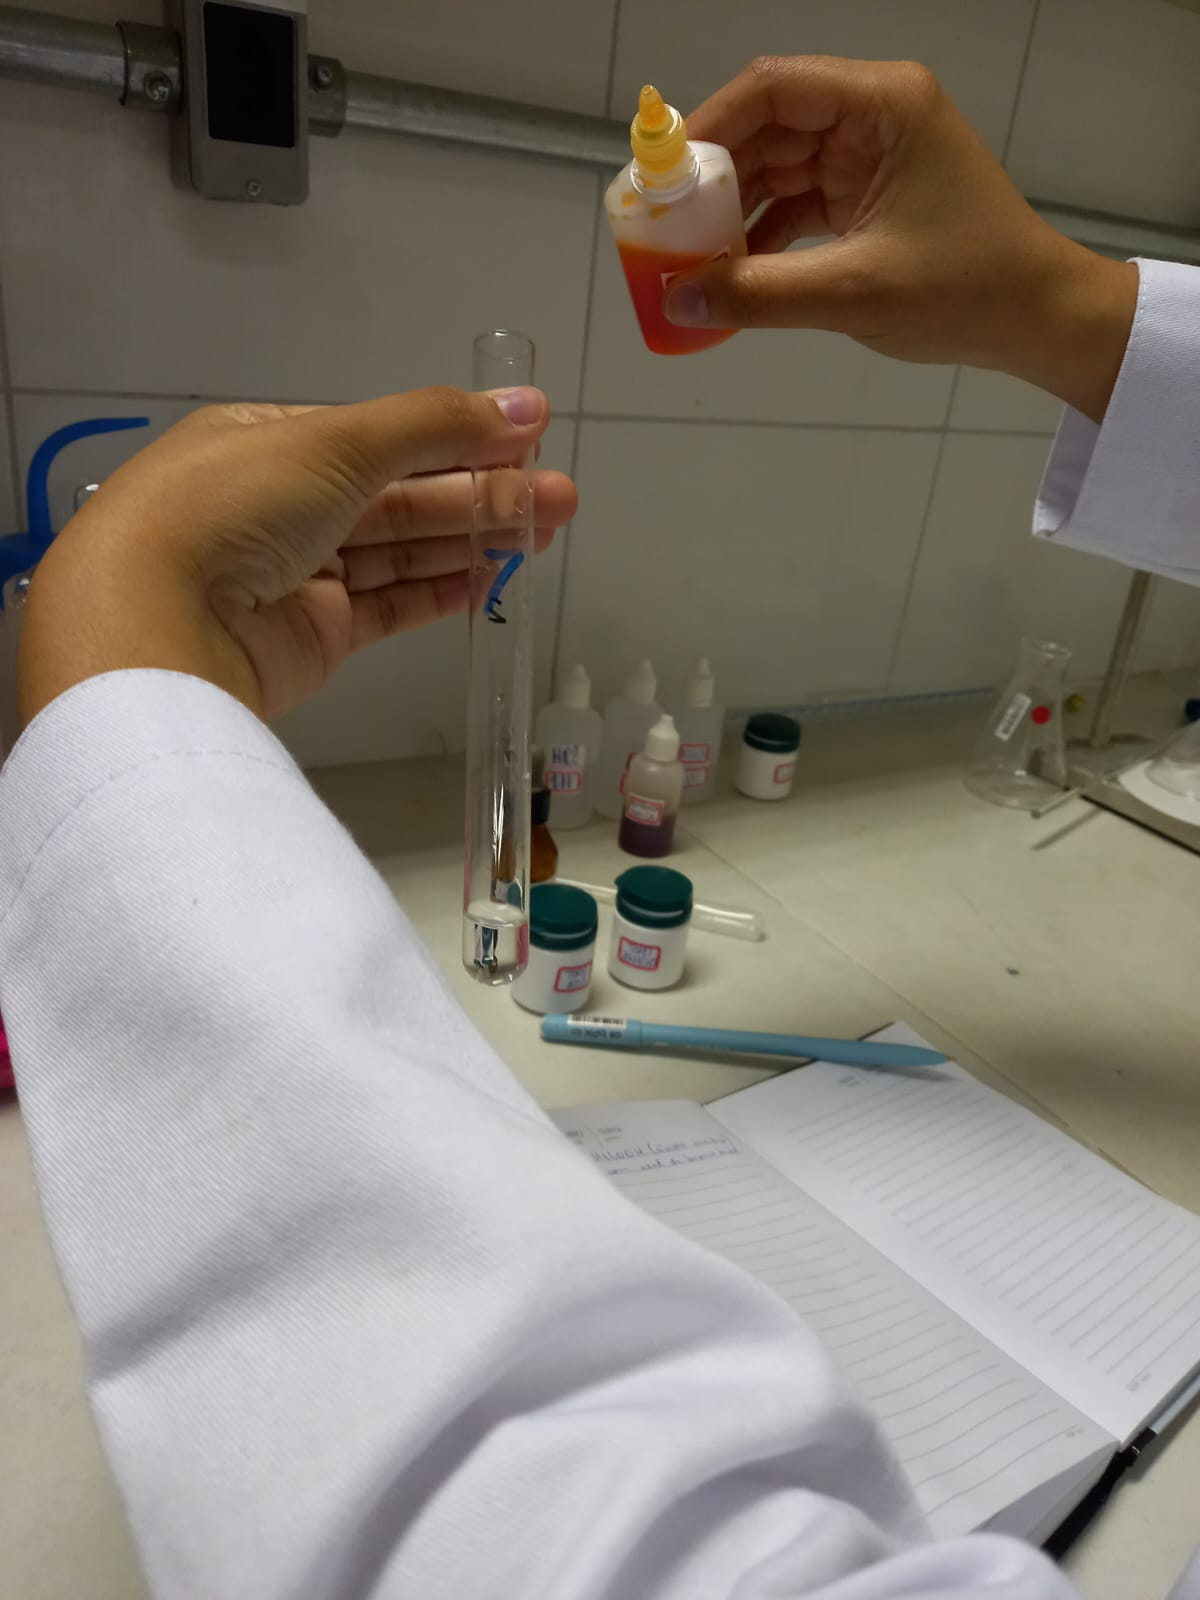
\includegraphics[scale=0.16]{pictures/tubo7pre.jpeg}}
            \qquad
            \subfloat[\centering A coloração apresentada pelo indicador foi amarela.\label{fig:figure14}]{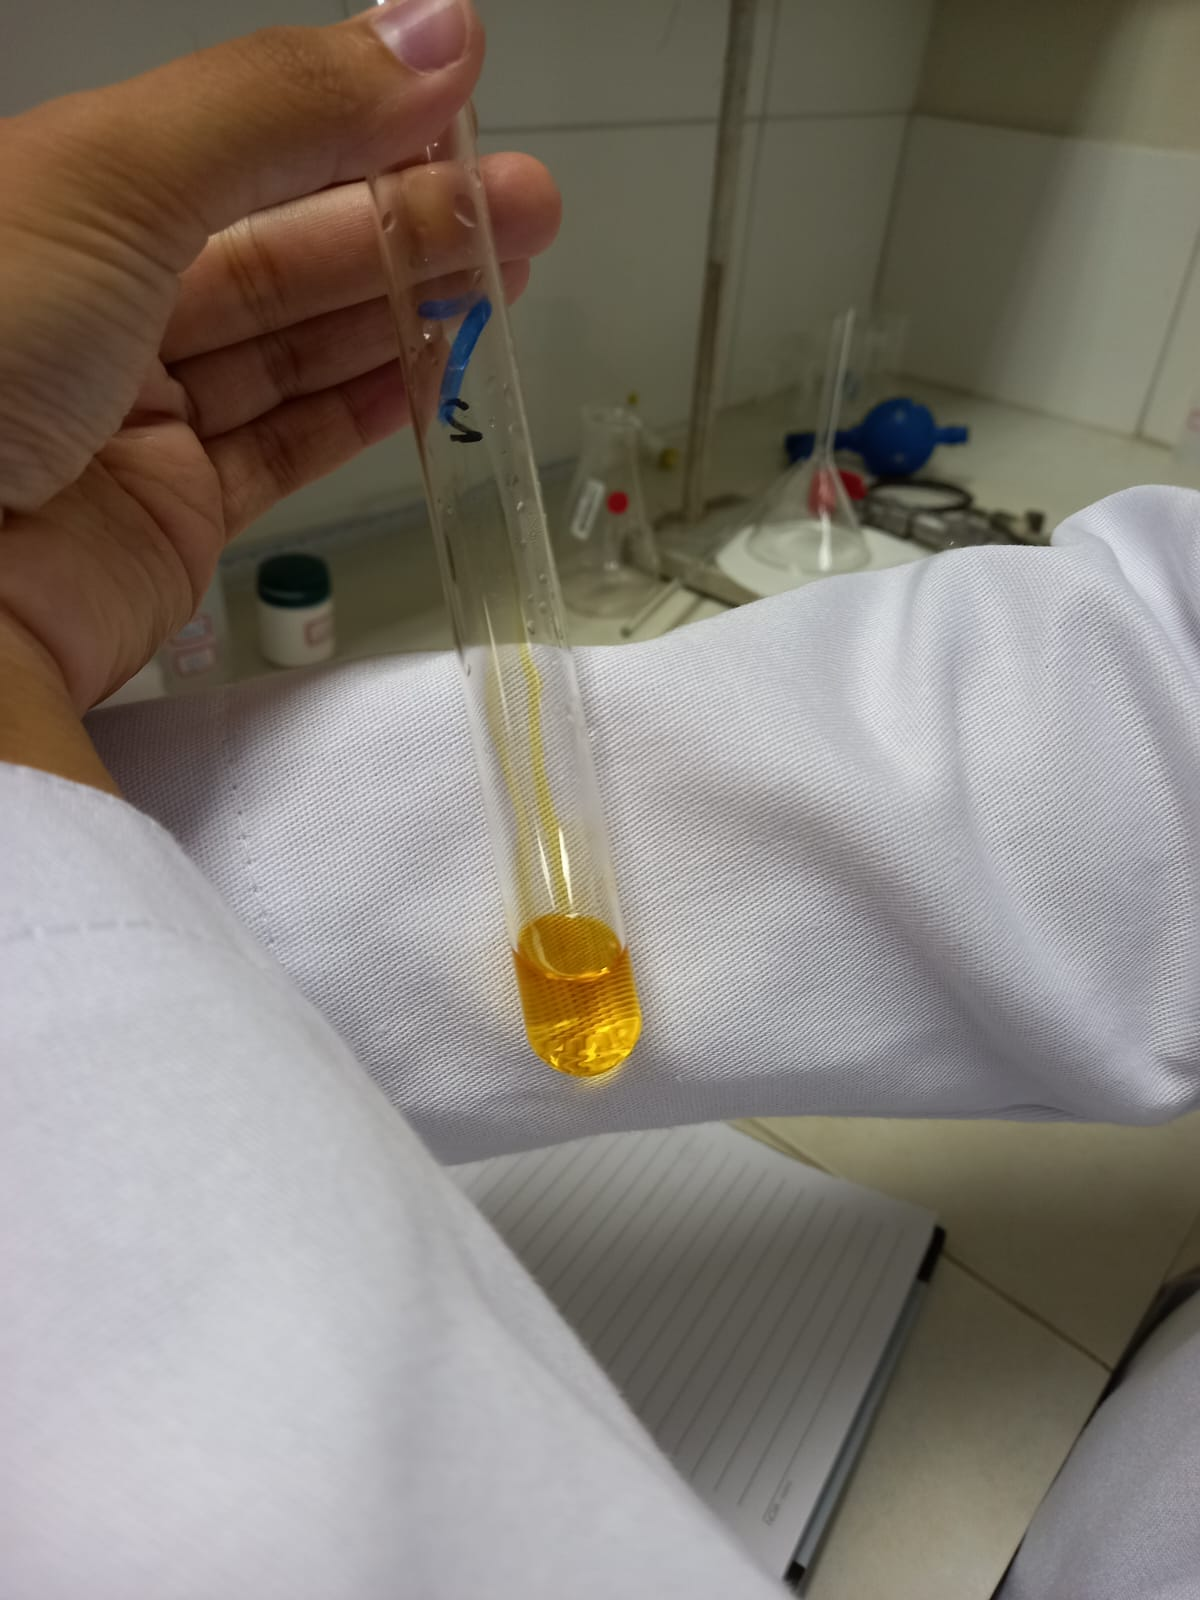
\includegraphics[scale=0.16]{pictures/tubo7pos.jpeg}}\label{fig:experimento16}
        \end{figure}
    
    	\indent Neste ensaio, houve o teste do indicador Azul Bromotimol com uma solução de ácido acético, sendo este indicador, tratado como um indicador universal para a identificação de soluções de caráter ácido, básico ou neutro, sendo que, para soluções ácidas, o mesmo apresenta coloração amarelada, em soluções básicas, a cor apresentada é azul, e em soluções de pH neutro, a cor apresentada é verde.\\
    	
    	\indent Como observado no experimento, ao entrar em contato com o ácido acético, o azul bromotimol adquiriu coloração amarela, e sendo assim, classificado como uma solução ácida.

    \newpage
	\subsubsection{Tubo de Ensaio 8}	
        \indent O oitavo tubo foi preparado com a solução de NH$_4$OH 0,1 mol/L, e foi testado com o indicador de pH, o azul de bromotimol, o qual apresentou uma cor amarela.

        \begin{figure}[h]
            \centering
            \subfloat[\centering Teste do indicador de pH com a solução de NH$_4$OH de 0,1 mol/L\label{fig:figure15}]{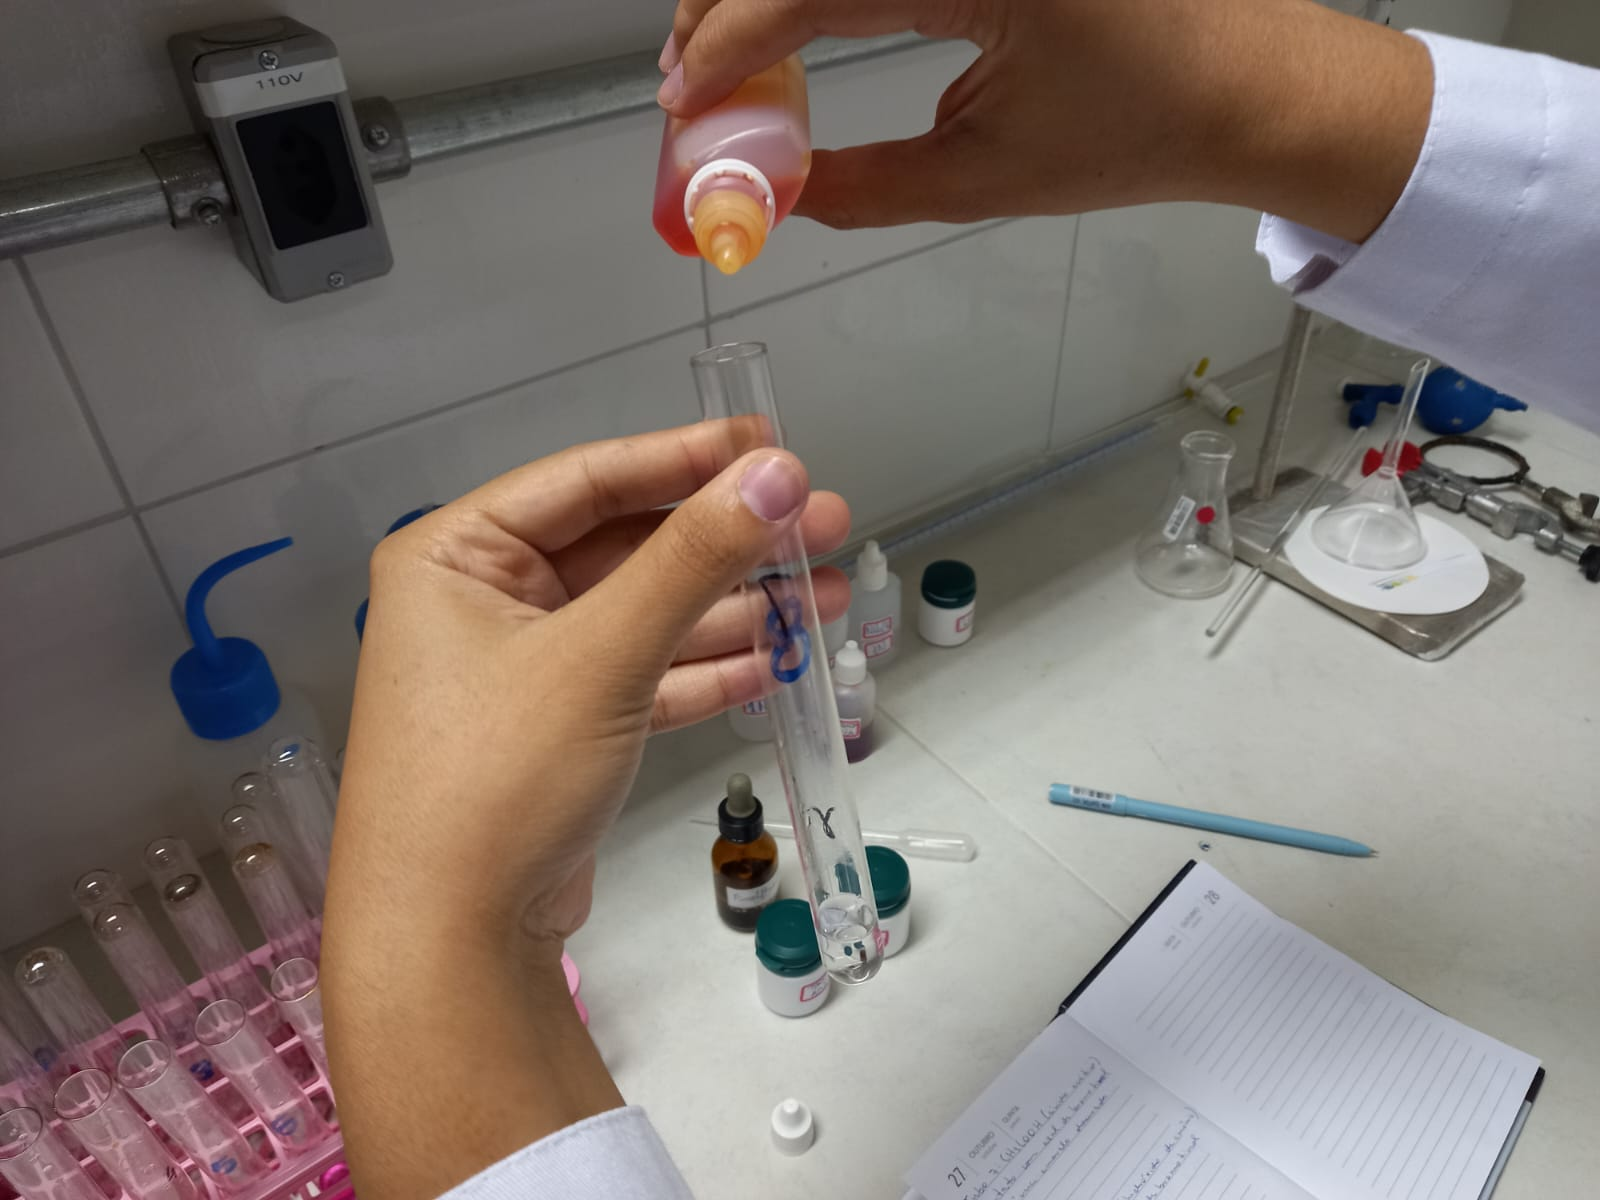
\includegraphics[scale=0.20]{pictures/tubo8pre.jpeg}}
            \qquad
            \subfloat[\centering A coloração apresentada pelo indicador foi azul.\label{fig:figure16}]{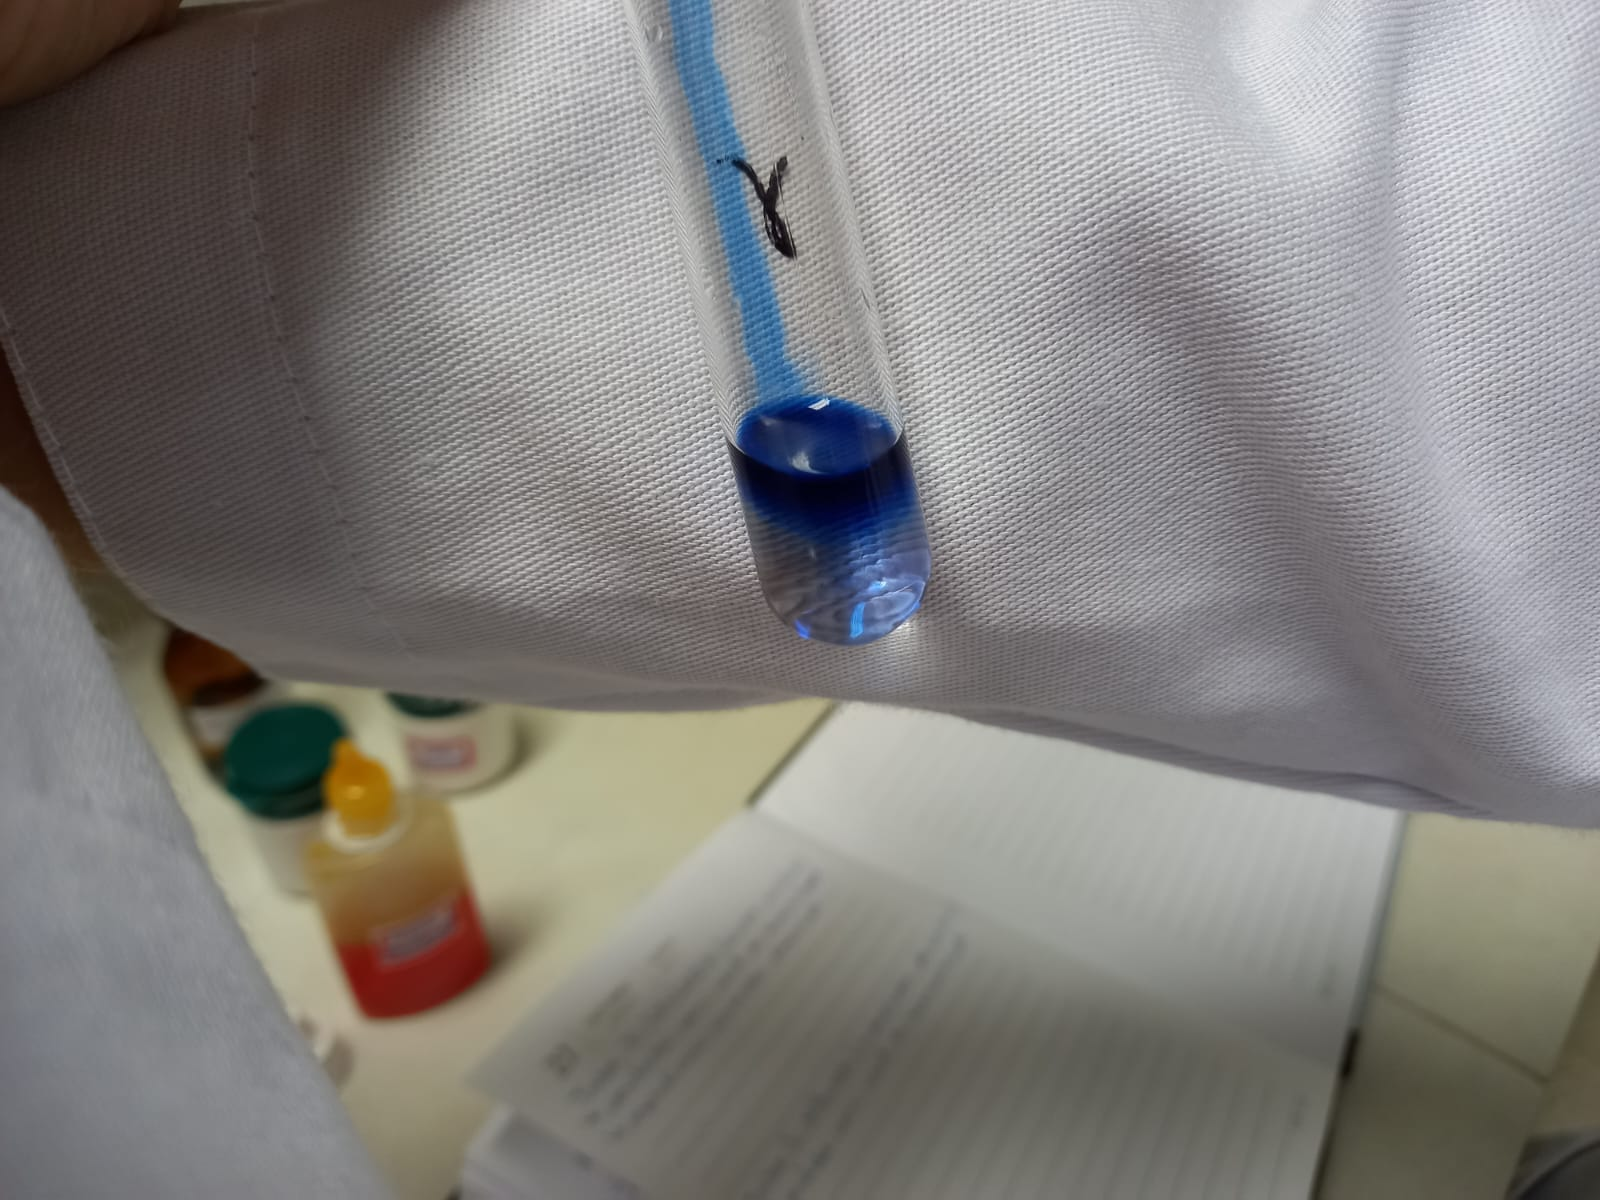
\includegraphics[scale=0.20]{pictures/tubo8pos.jpeg}}\label{fig:experimento17}
        \end{figure}
    
    	\indent Este foi mais um experimento utilizando o azul bromotimol como indicador para pH da solução. A solução em questão é o hidróxido de amônio, onde esta foi preparada no tubo de ensaio 8. \\
    	
    	\indent Como comentado no texto do tubo de ensaio 7, o azul bromotimol apresenta a tonalidade azul quando em contato com bases, e tal comportamento foi confirmado com a experimentação, onde a solução apresentou uma forte tonalidade azul.

        \newpage
        
        \subsection{Experimento 2: Comportamento de Produtos Comerciais em Presença de Indicadores}\label{subsubsec:mat_metodos_exp2}
        \indent Para a realização deste experimento, foi necessário obter alguns materiais para exemplo, dentre os quais, foram reunidos: Detergente, Água Sanitária, Suco de Limão, Suco de Uva e Água da Torneira.
        
        \begin{figure}[h]
        	\centering
        	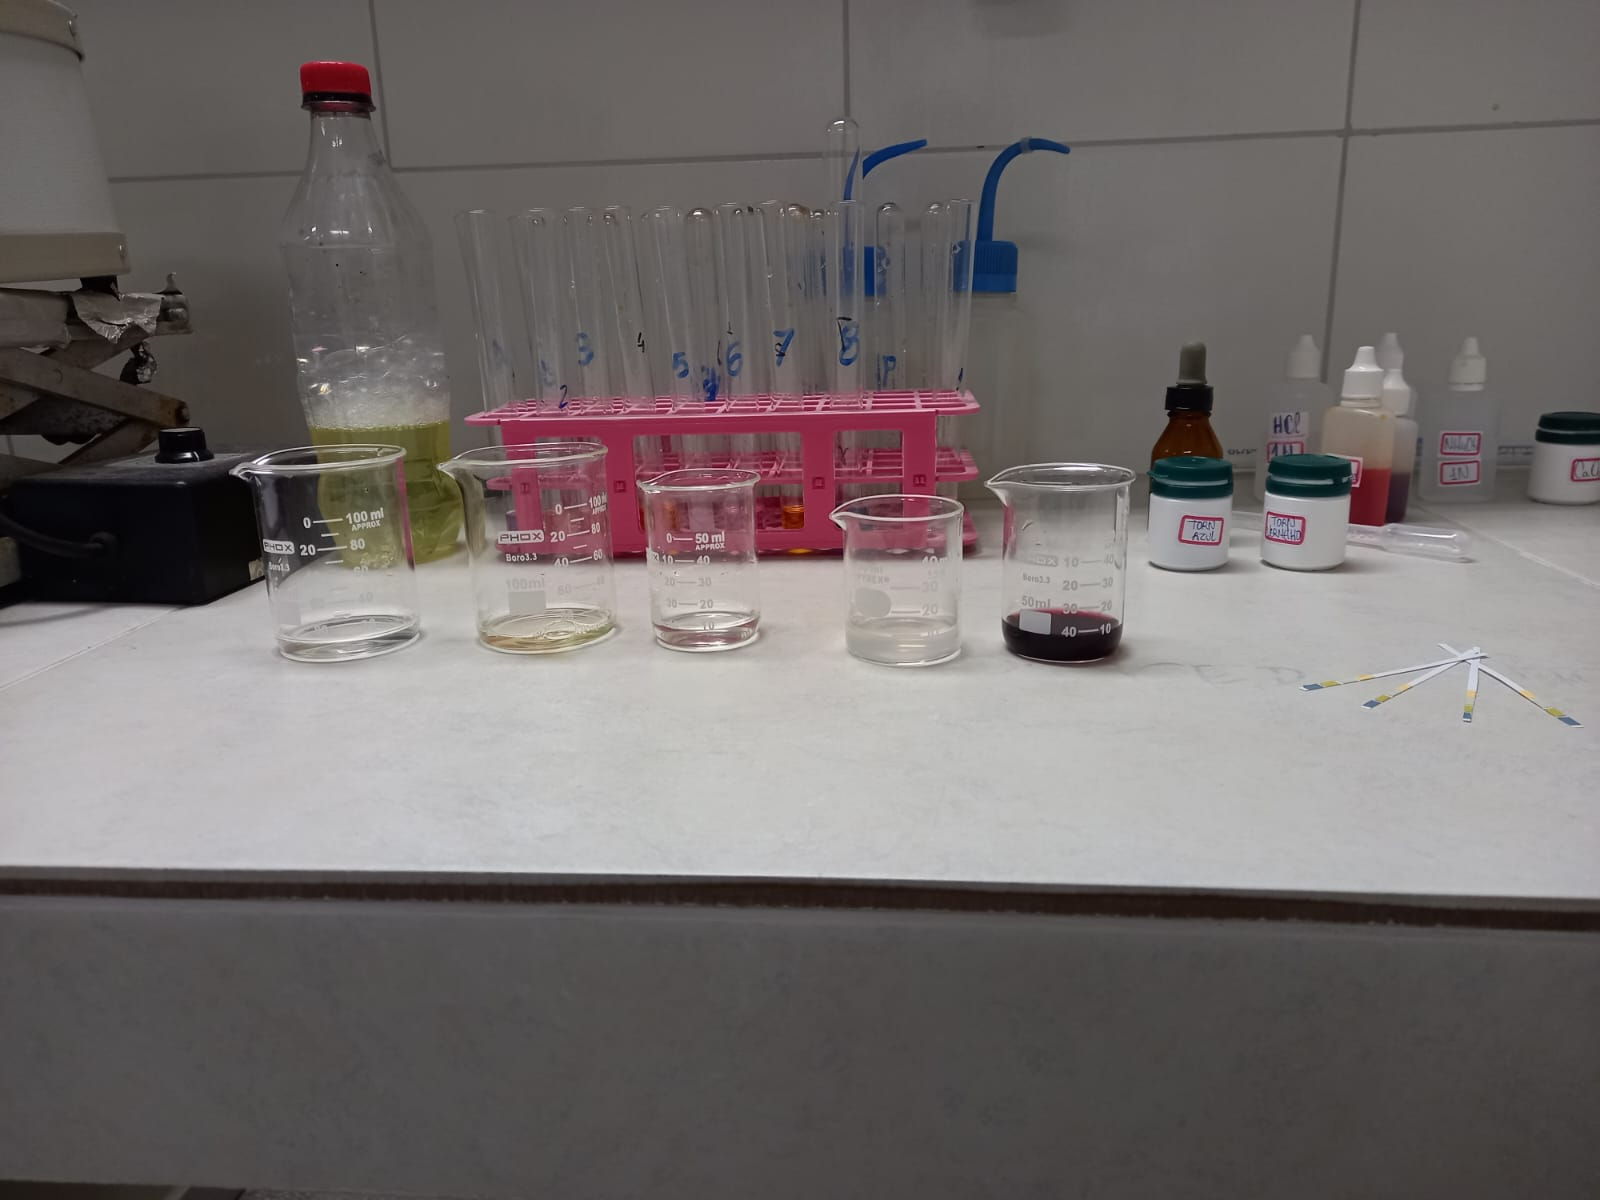
\includegraphics[scale=0.25]{pictures/bancada.jpeg}
        	\caption{Bancada com os materiais do segundo experimento}
        	\label{fig: Bancada do segundo experimento}
        \end{figure}
    %%%%%%%%%%%%%%%%%%%%%%%%%%%%%%%%%%%%%%%%%%%%%%%%%%%%%%%%%%%%%%%%%%%%%%%
    
        \subsubsection{Água de torneira}\label{exp2:aguatorneira}

            \indent A água que chega às nossas torneiras e abastece nossas cidades vem de reservatórios de água doce na superfície ou no subsolo, conhecidos como nascentes. No entanto, a maioria dessas nascentes acaba ficando imprópria para consumo devido ao tratamento de esgoto e efluentes industriais, poluentes, falta de planejamento e desmatamento.\\

            \indent Assim, antes de chegar à nossa casa, a água da nascente percorre longas distâncias e passa por uma série de tratamentos, pronta para beber. Esses tratamentos e adequações às normas vigentes são realizados em estações de tratamento de água (ETAs), que envolvem o controle e a correção do pH.\\

            \indent Os principais componentes da água comum tratada e utilizada em atividades domésticas são: alumínio, bário, cloro, ferro, fluoreto, nitratos, sódio, sulfato, entre outros. A água de torneira costuma possuir pH neutro, abaixo disso é considerado ácido já pH acima de 7 é básico ou alcalino. Por meio de nossa experiência praticada em laboratório, foi realizada a medida de pH com o uso de uma tira universal em contato com água retirada da torneira no momento da realização da atividade, e desse modo, verificamos que através da comparação entre as cores da tira utilizada e a tabela de pH, foi constatado que a água estava neutra com pH igual a 7.\\

        \subsubsection{Detergente}\label{exp2:Detergente}

            \indent Os detergentes são substâncias orgânicas formadas sinteticamente (em laboratório) cuja principal característica é a capacidade de facilitar a limpeza através de sua ação emulsificante, ou seja, a capacidade de facilitar a dissolução de substâncias. Os detergentes mais comuns são aqueles que contêm sulfonatos em sua estrutura, os reagentes utilizados na produção de tais detergentes são ácidos sulfônicos e quaisquer bases inorgânicas. Os detergentes neutros são os mais populares e conhecidos no mercado, são recomendados para limpeza do dia a dia e é ideal para remoção de sujidades mais leves ou então menores volumes de sujeiras. Os detergentes alcalinos possuem pH superior a 7 (em uma escala de 0 a 14). Eles removem todo tipo de sujeira, exceto as de origem mineral. Os detergentes neutros possuem pH próximo de 7, no ponto de equilíbrio entre acidez e alcalinidade.\\

            \indent Na experiência praticada em laboratório, foi realizada a medida de pH com o uso de uma tira universal em contato com o detergente comum utilizado na lavagem de louças, e que em razão do seu uso ser em contato direto com a pele durante a limpeza, possui pH com valor igual a 7. Desse modo, verificamos através da comparação entre as cores da tira utilizada e a tabela de pH, a confirmação que a substância estava neutra com pH igual a 7.\\

        \subsubsection{Água Sanitária}\label{exp2:aguasanitaria}

            \indent A solução de hipoclorito de sódio (NaClO), popularmente conhecida como água sanitária, é comumente utilizada na higienização de ambientes, pois, quando diluída em água, forma o ácido hipocloroso (HClO), eficaz contra os microrganismos patogênicos. O composto químico Hipoclorito de sódio, de fórmula NaClO, é usado como desinfetante e como agente alvejante. A água sanitária é produzida pela reação de cloro com hidróxido de sódio, o cloro é borbulhado em um recipiente e, ao mesmo tempo, se introduz vagarosamente uma solução alcalina de hidróxido de sódio (soda cáustica). A reação entre os componentes dessa mistura dá origem ao hipoclorito. O hipoclorito é um forte agente oxidante, usado em ambientes domésticos para eliminar vírus e bactérias, uma vez que estes são extremamente sensíveis à oxidação. Alvejantes se tornam eficientes para esterilizar a superfície das cozinhas, roupa suja, pias e banheiros.\\

            \indent Durante nossa experiência realizada em laboratório, foi feita a medida de pH com o uso de uma tira universal em contato com a água sanitária, no entanto, o cloro ativo presente na substância deteriorou os extratos de plantas contidos na fita universal e, dessa forma, se tornando esbranquiçado, perdendo gradativamente sua coloração. Logo não foi possível fazer a medição correta do pH da água sanitária.\\

        \subsubsection{Suco de limão}

            \indent O ácido cítrico presente no limão é um ácido orgânico tricarboxílico que está em grande parte das frutas, em especial nas ácidas e ele representa de 5 a 7\% da fruta. A molécula de ácido cítrico tem uma cadeia curta de 3 carbonos, comprimida por 3 volumosos grupos carboxila (-COOH), logo, trata-se de um ácido tricarboxílico. Algumas de suas propriedades são: fixação de cátions como cálcio, ferro, potássio e magnésio, agente de estabilização do pH de meios aquosos, sendo ele o principal agente de alcalinização do metabolismo orgânico de homens e animais, entre outros. Dessa forma, cumpre papel importante na estabilização do pH dos líquidos corporais, na eletroquímica (comunicação celular) do cérebro e de todo o organismo, no sistema de formação e manutenção óssea, na respiração celular e em toda a geração de energia da vida humana.\\

            \begin{figure}[h]
                \centering
                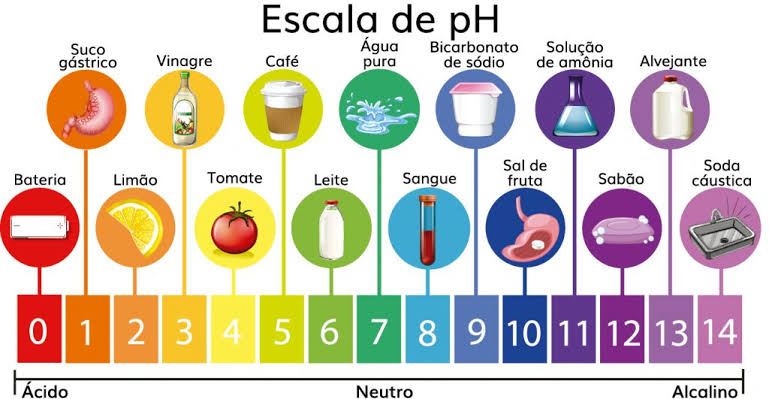
\includegraphics[width=0.8\textwidth]{pictures/schematic}
                \caption{Figura 5: Escala de pH}
                \label{fig:esquema}
            \end{figure}

            \indent Na experiência praticada em laboratório, foi realizada a medida de pH com o uso de uma tira universal em contato com o suco de limão artificial. Em pouco tempo após o contato entre a tira e a substância, foi observada a coloração correspondente a sua acidez. Desse modo, verificamos através da comparação entre as cores da tira utilizada e a tabela de pH, a confirmação que a substância estava ácida com pH igual a 2.\\

        \subsubsection{Suco de uva}\label{exp2:sucodeuva}
            \indent A uva é formada por compostos químicos representados principalmente por ésteres, terpenos, álcoois, ácidos, aldeídos e cetonas (carbonílicos), além de fonte de vitamina C. Tanto os taninos quanto o resveratrol são substâncias encontradas na casca das uvas e também de algumas outras frutas, que servem para protegê-las, naturalmente, contra pragas, fungos e insetos. Mas a uva possui uma grande quantidade de polifenóis, incluindo resveratrol, ácidos fenólicos, antocianinas e flavonóides, que são compostos antioxidantes. Todas essas substâncias estão presentes no suco de uva integral, que é produzido com a fruta inteira, incluindo cascas e sementes. Porém, alguns produtos conhecidos como néctar não têm a mesma composição. Normalmente, contam com adição de outros ingredientes (como suco de maçã, soja e açúcar) e podem conter aditivos químicos, como conservantes, corantes e flavorizantes.\\

            \indent O suco de uva possui pH entre 3 e 4, logo, levemente ácido. No entanto, sua visualização é dificultada em razão de sua cor se sobrepor a cor dos indicadores. A nossa experiência demonstrou esse fato já que durante a realização  da medida de pH com o uso de uma tira universal em contato com o suco, não foi possível observar a coloração correspondente na tabela de pH, já que a tonalidade da substância prejudicou a pigmentação da tira universal, desse modo, nesse caso não foi possível obter uma resposta com relação ao pH do suco de uva usado no experimento.\\
		
		\newpage
        \section{Conclusão}\label{exp2:conclusão}
            \indent Foi possível preparar o experimento químico verificando o valor de pH de diferentes substâncias, seguindo os procedimentos de segurança conforme os parâmetros recomendados. A equipe obteve boa experiência prática e técnica, registrando as observações sobre cada etapa do experimento. Obtivemos amplo aprendizado a cerca dos diferentes modos de verificação de pH, assim como, as características de diferentes substâncias e suas relações de acidez ou basicidade.\\
        
        \newpage


